% Options for packages loaded elsewhere
\PassOptionsToPackage{unicode}{hyperref}
\PassOptionsToPackage{hyphens}{url}
%
\documentclass[
]{article}
\usepackage{amsmath,amssymb}
\usepackage{lmodern}
\usepackage{ifxetex,ifluatex}
\ifnum 0\ifxetex 1\fi\ifluatex 1\fi=0 % if pdftex
  \usepackage[T1]{fontenc}
  \usepackage[utf8]{inputenc}
  \usepackage{textcomp} % provide euro and other symbols
\else % if luatex or xetex
  \usepackage{unicode-math}
  \defaultfontfeatures{Scale=MatchLowercase}
  \defaultfontfeatures[\rmfamily]{Ligatures=TeX,Scale=1}
\fi
% Use upquote if available, for straight quotes in verbatim environments
\IfFileExists{upquote.sty}{\usepackage{upquote}}{}
\IfFileExists{microtype.sty}{% use microtype if available
  \usepackage[]{microtype}
  \UseMicrotypeSet[protrusion]{basicmath} % disable protrusion for tt fonts
}{}
\makeatletter
\@ifundefined{KOMAClassName}{% if non-KOMA class
  \IfFileExists{parskip.sty}{%
    \usepackage{parskip}
  }{% else
    \setlength{\parindent}{0pt}
    \setlength{\parskip}{6pt plus 2pt minus 1pt}}
}{% if KOMA class
  \KOMAoptions{parskip=half}}
\makeatother
\usepackage{xcolor}
\IfFileExists{xurl.sty}{\usepackage{xurl}}{} % add URL line breaks if available
\IfFileExists{bookmark.sty}{\usepackage{bookmark}}{\usepackage{hyperref}}
\hypersetup{
  pdftitle={iSEGMound -- a Reproducible Workflow for Mound Detection in LiDAR-derived DTMs},
  pdfauthor={Submitted in accordance with the requirements for the degree of Master of Science; Philipps-University Marburg; Department of Physical Geography},
  hidelinks,
  pdfcreator={LaTeX via pandoc}}
\urlstyle{same} % disable monospaced font for URLs
\usepackage[margin=1in]{geometry}
\usepackage{color}
\usepackage{fancyvrb}
\newcommand{\VerbBar}{|}
\newcommand{\VERB}{\Verb[commandchars=\\\{\}]}
\DefineVerbatimEnvironment{Highlighting}{Verbatim}{commandchars=\\\{\}}
% Add ',fontsize=\small' for more characters per line
\usepackage{framed}
\definecolor{shadecolor}{RGB}{248,248,248}
\newenvironment{Shaded}{\begin{snugshade}}{\end{snugshade}}
\newcommand{\AlertTok}[1]{\textcolor[rgb]{0.94,0.16,0.16}{#1}}
\newcommand{\AnnotationTok}[1]{\textcolor[rgb]{0.56,0.35,0.01}{\textbf{\textit{#1}}}}
\newcommand{\AttributeTok}[1]{\textcolor[rgb]{0.77,0.63,0.00}{#1}}
\newcommand{\BaseNTok}[1]{\textcolor[rgb]{0.00,0.00,0.81}{#1}}
\newcommand{\BuiltInTok}[1]{#1}
\newcommand{\CharTok}[1]{\textcolor[rgb]{0.31,0.60,0.02}{#1}}
\newcommand{\CommentTok}[1]{\textcolor[rgb]{0.56,0.35,0.01}{\textit{#1}}}
\newcommand{\CommentVarTok}[1]{\textcolor[rgb]{0.56,0.35,0.01}{\textbf{\textit{#1}}}}
\newcommand{\ConstantTok}[1]{\textcolor[rgb]{0.00,0.00,0.00}{#1}}
\newcommand{\ControlFlowTok}[1]{\textcolor[rgb]{0.13,0.29,0.53}{\textbf{#1}}}
\newcommand{\DataTypeTok}[1]{\textcolor[rgb]{0.13,0.29,0.53}{#1}}
\newcommand{\DecValTok}[1]{\textcolor[rgb]{0.00,0.00,0.81}{#1}}
\newcommand{\DocumentationTok}[1]{\textcolor[rgb]{0.56,0.35,0.01}{\textbf{\textit{#1}}}}
\newcommand{\ErrorTok}[1]{\textcolor[rgb]{0.64,0.00,0.00}{\textbf{#1}}}
\newcommand{\ExtensionTok}[1]{#1}
\newcommand{\FloatTok}[1]{\textcolor[rgb]{0.00,0.00,0.81}{#1}}
\newcommand{\FunctionTok}[1]{\textcolor[rgb]{0.00,0.00,0.00}{#1}}
\newcommand{\ImportTok}[1]{#1}
\newcommand{\InformationTok}[1]{\textcolor[rgb]{0.56,0.35,0.01}{\textbf{\textit{#1}}}}
\newcommand{\KeywordTok}[1]{\textcolor[rgb]{0.13,0.29,0.53}{\textbf{#1}}}
\newcommand{\NormalTok}[1]{#1}
\newcommand{\OperatorTok}[1]{\textcolor[rgb]{0.81,0.36,0.00}{\textbf{#1}}}
\newcommand{\OtherTok}[1]{\textcolor[rgb]{0.56,0.35,0.01}{#1}}
\newcommand{\PreprocessorTok}[1]{\textcolor[rgb]{0.56,0.35,0.01}{\textit{#1}}}
\newcommand{\RegionMarkerTok}[1]{#1}
\newcommand{\SpecialCharTok}[1]{\textcolor[rgb]{0.00,0.00,0.00}{#1}}
\newcommand{\SpecialStringTok}[1]{\textcolor[rgb]{0.31,0.60,0.02}{#1}}
\newcommand{\StringTok}[1]{\textcolor[rgb]{0.31,0.60,0.02}{#1}}
\newcommand{\VariableTok}[1]{\textcolor[rgb]{0.00,0.00,0.00}{#1}}
\newcommand{\VerbatimStringTok}[1]{\textcolor[rgb]{0.31,0.60,0.02}{#1}}
\newcommand{\WarningTok}[1]{\textcolor[rgb]{0.56,0.35,0.01}{\textbf{\textit{#1}}}}
\usepackage{longtable,booktabs,array}
\usepackage{calc} % for calculating minipage widths
% Correct order of tables after \paragraph or \subparagraph
\usepackage{etoolbox}
\makeatletter
\patchcmd\longtable{\par}{\if@noskipsec\mbox{}\fi\par}{}{}
\makeatother
% Allow footnotes in longtable head/foot
\IfFileExists{footnotehyper.sty}{\usepackage{footnotehyper}}{\usepackage{footnote}}
\makesavenoteenv{longtable}
\usepackage{graphicx}
\makeatletter
\def\maxwidth{\ifdim\Gin@nat@width>\linewidth\linewidth\else\Gin@nat@width\fi}
\def\maxheight{\ifdim\Gin@nat@height>\textheight\textheight\else\Gin@nat@height\fi}
\makeatother
% Scale images if necessary, so that they will not overflow the page
% margins by default, and it is still possible to overwrite the defaults
% using explicit options in \includegraphics[width, height, ...]{}
\setkeys{Gin}{width=\maxwidth,height=\maxheight,keepaspectratio}
% Set default figure placement to htbp
\makeatletter
\def\fps@figure{htbp}
\makeatother
\setlength{\emergencystretch}{3em} % prevent overfull lines
\providecommand{\tightlist}{%
  \setlength{\itemsep}{0pt}\setlength{\parskip}{0pt}}
\setcounter{secnumdepth}{5}
\ifluatex
  \usepackage{selnolig}  % disable illegal ligatures
\fi

\title{iSEGMound -- a Reproducible Workflow for Mound Detection in LiDAR-derived DTMs}
\usepackage{etoolbox}
\makeatletter
\providecommand{\subtitle}[1]{% add subtitle to \maketitle
  \apptocmd{\@title}{\par {\large #1 \par}}{}{}
}
\makeatother
\subtitle{Agnes Schneider}
\author{Submitted in accordance with the requirements for the degree of Master of Science\textsuperscript{} \and Philipps-University Marburg\textsuperscript{} \and Department of Physical Geography\textsuperscript{}}
\date{16.09.2021}

\begin{document}
\maketitle

{
\setcounter{tocdepth}{2}
\tableofcontents
}
\newpage

\hypertarget{acknowlegements}{%
\section*{Acknowlegements}\label{acknowlegements}}
\addcontentsline{toc}{section}{Acknowlegements}

\newpage

\pagenumbering{arabic}

\hypertarget{introduction}{%
\section{Introduction}\label{introduction}}

The use of quantitative methods in archaeology reach back to the end of the 19th century, but it was only after the middle of the 20th century that they became computer-based. The first applications of statistical-mathematical methods using computers revolutionized the handling of spatial and quantitative archaeological data (e.g.~Goldmann 1979) and also the view on archaeology itself (e.g.~Clark 1968 and almost a decade later Hodder and Orton 1976, Ihm and Zimmermann 1978 to begin with). This quantitative analytical view preceded and prepared archaeologists for the advent of the public availability of soon high resolution digital datasets which revolutionized and broadened Aerial Archaeology, drawing upon the expertise of Satellite Remote Sensing and branching into a new discipline: Archaeological Remote Sensing. These new data sources, including geophysical platforms, led to the need to handle - in archaeological terms - big spatial data, thus to the specialized use of GIS platforms and the development and application of new methods like predictive modelling (van Leusen -- Kamermans 2005; Kamermans et al.~2009). The sophistication of airborne platforms, sensors and imaging technologies, like LiDAR, hyper-spectral imagery and drone derived multispectral and hyper-spectral imagery (Agapiou -- Lysandrou 2015; Luo et al.~2019) facilitated the diversification of the toolset of Archaeological Remote Sensing.
New technical developments continuously push specialists to look for, borrow and adapt new methods to analyse in archaeological sense big data, which first lead to automating tasks such as georeferencing or applying the same function on multiple rasters (Raun and Patterson 2018, 70). Soon this lead to more complex automation -- that is automating whole workflows and also analysis.
Thus in contrast to other disciplines, Archaeological Remote Sensing and Archaeological Science itself was quite late in adopting and applying automated methods and thus, Automated Archaeological Remote Sensing is still in its infancy (Opitz and Herrmann 2018, 30). Although accordingly, the expression `automated analysis' is still controversial, it is nonetheless used throughout this Master's thesis. It has to be emphasized that `automation' does not stand for completely automated workflows. It was chosen as a short phrase to address workflows with at least partly -- or mostly -- automated elements, because no one advocates `automatic archaeology' (Cowley 2012, 6). Automated analysis, often also called semi-automated analysis, `simply' means that a part, often a major part of a specific workflow, is automated, meaning computer aided.
Critical voices about predictive modelling in GIS ˗ which can be seen as the precursor and actual starting point of automated analysis ˗ were very fittingly summarized by Wheatley 2004: predictive modelling is dehumanising, anti-historical and substitutes human actions with mathematical equations (Wheatley 2004). This distrust is reflected in the criticism towards automated analysis methods in the Archaeological and Archaeological Remote Sensing community, claiming, that archaeological projects are always locally specialized (Parcak 2009, 120) and that there is no generalized automation method that can be used location independently, which can locate atypical archaeological objects without producing a quite large miss-rate (Casana 2014, Casana 2020, S93). Taking these points into account: why only use one type of automated analysis method (Davis 2019, 5)? Large-scale landscapes feature lots of different landscape forms and archaeological features which need to be addressed in different ways. It is evident that it is not possible to detect everything with one analysis method or algorithm, due to the variability of the archaeological record. Other considerations include reflections on Automated Archaeological Remote Sensing detecting round and square shapes over and over and when it will move to something more useful that actually resembles archaeological objects (Rog Palmer in personal discussion and several AARGnews Editorials and contributions, e.g.~AARGnews 62, 61)?
It is also somehow self-evident, that although pre-trained and known object classes are going to be detected, new and unexpected and also not detected objects always have to be expected. Thus expecting to detect unexpected or unknown object classes with supervised learning/automation is misleading and completely unrealistic (see a similar discussion about the use of predictive modelling in Wheatley 2004, 3.2.3). It is a fatal move to expect automation to be the magic trick, when it is not: it should be more seen as an extension of the archaeologist's toolbox. Because automated analysis is not to replace manual data evaluation which, based on the personal experience of the operator and them being human, can be prone to missing knowledge or error, or even archaeologists completely, but to be complementary. Automated analysis should be followed by field observation and identification for assessment, which on the other hand also can be biased for the same reason as manual data evaluation (Cowley 2012, Bennett et al 2014, 899). All in all automated analysis is to ease and facilitate the amount of work archaeologists are facing with the increasing amount of data and different data types to analyse and evaluate. As Davis (2020a, 3) emphasizes: automated analysis is precise and manual analysis is accurate. Thus both methods combined can help archaeologists to penetrate a hidden level of any dataset and landscape, which is invisible or hardly visible even for the trained eye.
Taking it further, reproducible analysis (Marwick 2017, Rokem et al.~2017, Marwick et al.~2018, Calero Valdez 2020) can help to facilitate automated analyses and can serve as control for human individuality: because archaeologists do see different things in the same data set and unconsciously see what they are familiar with and what they know (Cowley 2012, 7), very similarly to an algorithm trained to find a certain class of object. Human detection cannot be reproduced but automated analysis can: via documented, reproducible workflows. In order to achieve this goal open-source scripting languages like R, Python or open-source platforms like Google Engine should be used, to be able to repeat, reproduce and even replicate workflows to facilitate their use by other scholars. When writing code, the semantic syntax has to be clear and consistent. This also makes sure that the ontology and the semantic syntax will be the same when the code is used by a different operator on a different dataset -- in contrary to manual analysis, where independent, subjective manual operators would define features or objects differently -- thus arriving to the same or a least similar bias and errors, of course depending on the dataset. This argument is investigated more thoroughly in chapter III and the expressions reproducible and replicable are discussed in more detail.

Being entirely different disciplines, there is a semantic gap between the ontologies of Computer Vision, Image Analysis and Remote Sensing on one hand and Archaeology on the other hand -- especially because the archaeological record itself is fragmented, multifaceted and poses ontological problems in itself for the interoperability of projects or databases, conducted by different operators with possible different metalanguage. Although the aim of this thesis is not the creation of an ontological and semantic framework and/or a metalanguage for Automated Archaeological Remote Sensing, these points have to be discussed because they affect the way how automation can be harmonized with Archaeological Remote Sensing.\\
This fundamental difference is reflected in the fact, that a distinction has to be made between `object' and `feature' in sensu stricto automation, based on termini technici from Computer Vision, on which ground `object' is referred to real-world entities in remote sensing images and `feature' to elements of an image and of an object (Traviglia et al.~2016, 12; Lambers et al 2019, 2), in contrary to the every-day use of the expression `archaeological feature' at an excavation site or in reports. Reproducible code and workflows enable to conduct the same `procedure' in a controlled environment and thus possible semantic problems which can result from how different operators see archaeological objects and features can be detected, distinguished and solved. Thus the accurate expert knowledge of manual analysis can be integrated in the precision and consistency of computational semantics (Davis 2020a, Fig 1.).

\textbackslash begin\{figure\}

\{\centering 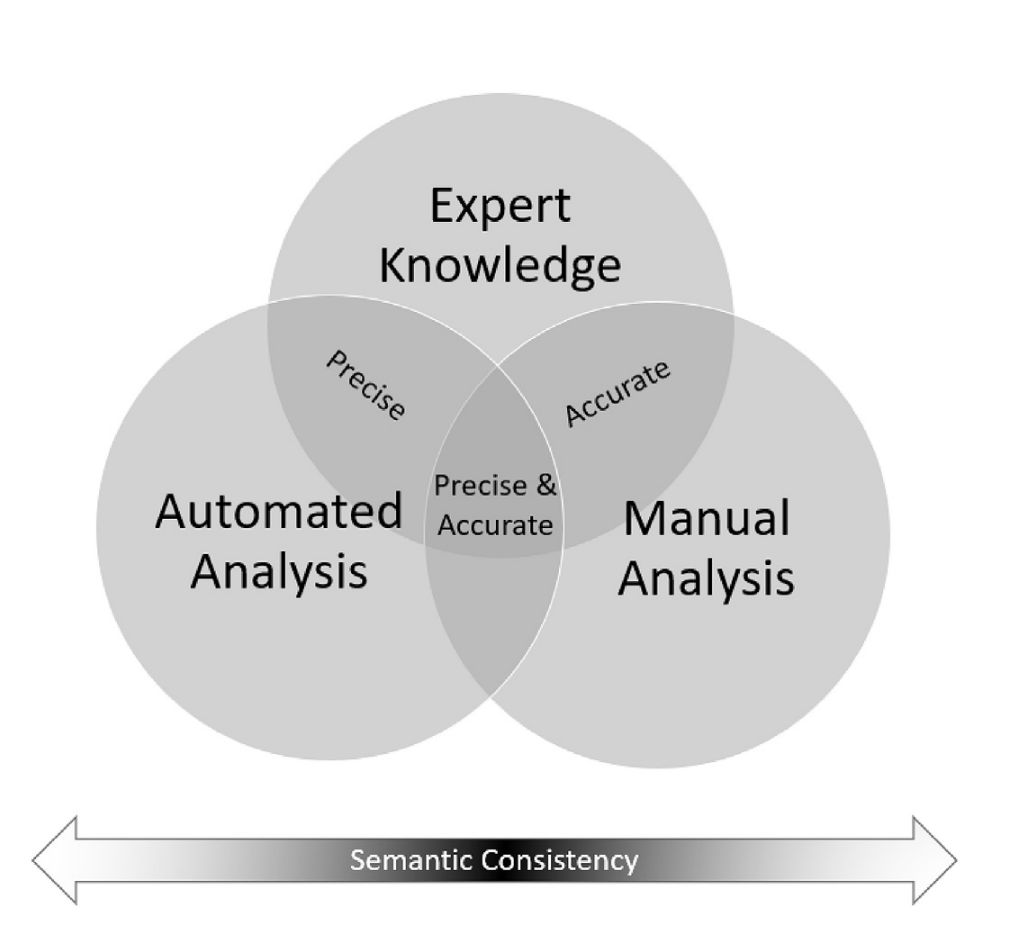
\includegraphics[width=0.5\linewidth,height=0.5\textheight]{C:/Users/kelto/Documents/iSEGMound/analysis/figures/Figure_1}

\}

\caption{Figure 1. Chart showing the advantages (approaching Semantic Consistency) when Expert Knowledge, Manual Analysis and Automated analysis are combined. Source: Davis 2020a, Fig 1.}

(\#fig:Figure\_1)
\textbackslash end\{figure\}

On the other hand, manual analysis can learn a lot from the systematic precision of reproducible code: defining variables, consistent nomenclature of objects/ forms/ features; creating functions: setting the relation of objects/ forms/ features. This needs the consistency of formalized, straightforward and clear definitions (also Magnini and Bettineschi 2019, 13, Davis 2020a). Thus ontology, semantics and metadata are very important tools which enable us to connect and share code, databases and research. By shared ontologies (knowledge representation), codified metalanguage protocols and rule-sets, not only would the transferability of expert knowledge be substantially eased between Archaeological disciplines and Automated Archaeological Remote Sensing, but also between its different subdisciplines, like Template Matching-, Geometric knowledge-, GeOBIA-, Machine Learning- based analyses (this distinction is explained in chapter 2).

So then, after all, how to semantically address the varying, unpredictable, fragmented, multifaceted and diachronic archaeological record (monuments and artefacts) which can be detected in remote sensing data with methods of Computer Vision and Image Analysis? Remote sensing data offers much more: they are diachronic time capsules, records of palimpsest landscapes, archaeological, micro- and macro-topographical, geomorphological and also recent, anthropomorphic traces (Magnini and Bettineschi 2019, 12) in a multidimensional space. Thus a common ground has to be created (a shared diachronic formalized ontology) to fill the semantic gap between the metalanguage of human perception, the archaeological record (which is manifold, imbalanced and changing in time (conceptually and physically) and Computer Vision/Image Analysis. And a way has to be found to apply this new diachronic formalized ontology onto real world scenarios (using Automated Archaeological Remote Sensing). Real world (archaeological) scenarios are often extremely complex and thus robust simplification and formalization has to be executed to break down complexity and bring the domains in discussion together. Sevara and Pregesbauer (2014) already pioneered a conceptual framework in 2014, which found resonance and the formulation of a Diachronic Semantic Model (DSM) in Magnini and Bettineschi 2019, which was successfully applied by the latter on a case study in 2021 (Magnini and Bettineschi 2021). These fundamental studies are the first steps towards integrating Automated Archaeological Remote Sensing in the nervous system of Archaeological Science.

As concluding thoughts let a quote from Quintus et al.~(2017, 1) state: \emph{``many archaeological professionals who might have an interest in lidar-derived products do not have the technical experience to modify or create AFE (automated feature extraction) techniques for particular regions or environments.''} This should not impact the scientific methods one chooses. With open-source, reproducible (regularly updated and version controlled) and code, with clear replicable workflows and published data and study (at least the manuscript in a preprint repository) (Figure 3), every remote sensing archaeological professional should be able to tap into the possibilities of Automated Analysis. Thus open access and open source software should be used, training data sets and workflows released to be able to learn from each other and to progress, building on the experience of each other and not to have to start from scratch with every new project conducted.

\textbackslash begin\{figure\}

\{\centering 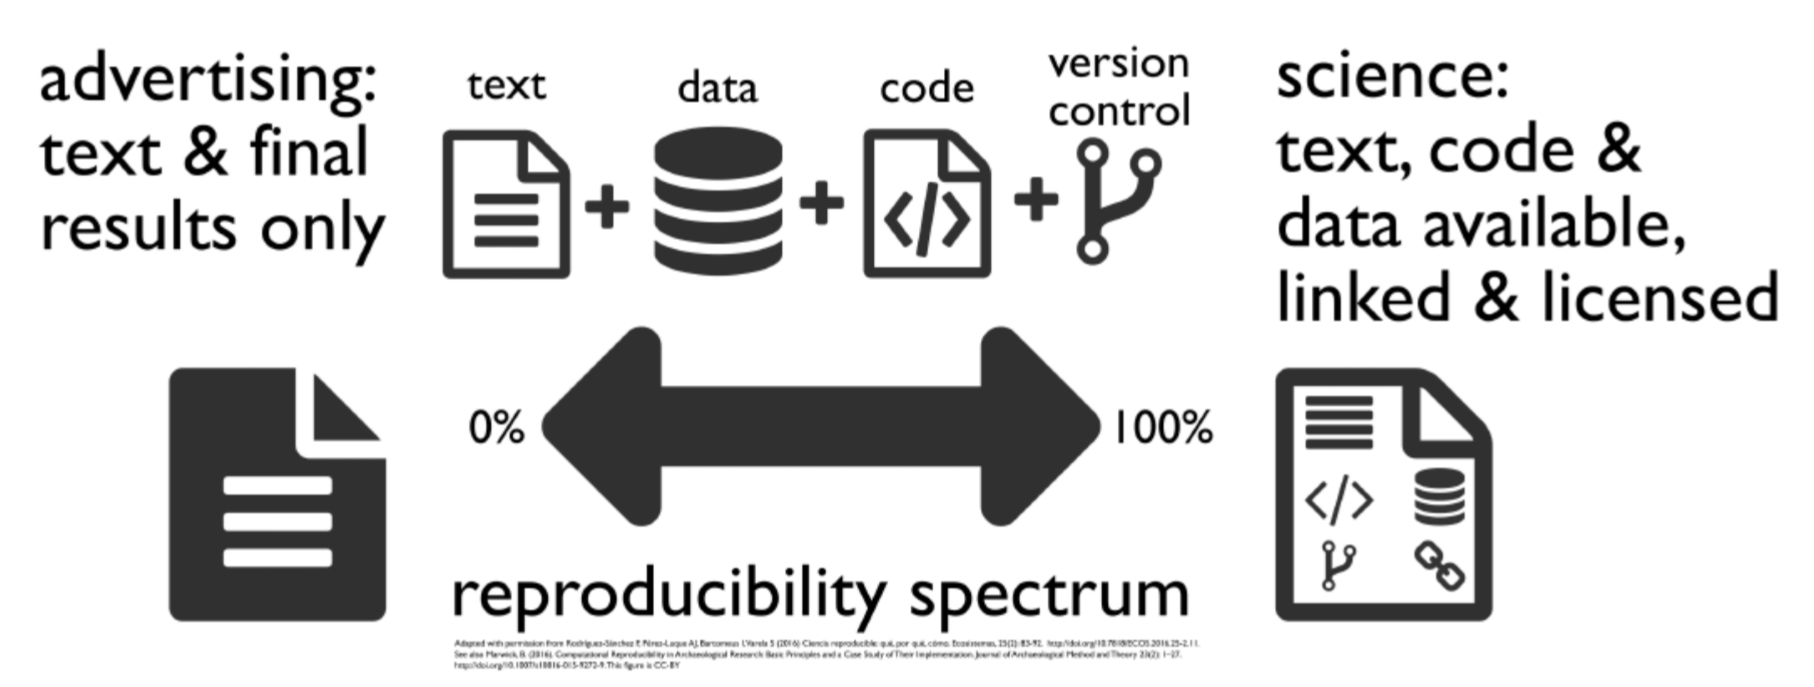
\includegraphics[width=0.75\linewidth,height=0.75\textheight]{C:/Users/kelto/Documents/iSEGMound/analysis/figures/Figure_2}

\}

\caption{Figure 2. The difference between articles behind paywall and reproducible (and replicable) studies. Source: Marwick et al. 2017, Figure 1.}

(\#fig:Figure\_2)
\textbackslash end\{figure\}

Thus we not only need to compare the accuracy and the true and false positive rate of different automated methods (Trier at al.~2018, Table 1) and the methods themselves (Davis et al.~2019), but we need to make a compendium of these methods with the key elements mentioned above. Combined with this, a baseline or best practice for the different methods should be defined that can be utilized by beginners. Thus open-access code, workflow and protocol, published (at least training) data sets and best practices are needed as reference and base line for other studies, stored in an open-source database or platform which can support open-source computer languages.

Different observations made above and questions based on these have led to the objective of this thesis. Firstly: based on scientific literature, on what grounds lies the dispute of automation in Archaeological Remote Sensing and how can it be relieved? Is the experience and knowledge gained transferable to other studies? How many scientific studies on burial mound detection worked transparently and retraceable (reproducible if not replicable) in any step of their workflow? Can experiences and knowledge from previous studies be used to create a reproducible and replicable workflow for burial mound detection?\\
Thus the aim of this Master's thesis is to emphasize the applicability and usefulness of automation in dealing with big datasets in Archaeological Remote Sensing and the need for reproducible and replicable workflows and studies. The case study for this thesis is the detection of burial mounds in LiDAR datasets in R, to substantiate this point of view.

To approach these questions accordingly, after the discussion of Automated Archaeological Remote Sensing and its reception in Archaeological Science was discussed in Chapter I, the Introduction. In the next chapter (II) all published studies whose goal is to detect burial mounds or mound-like structures are discussed in terms of used methods, software, accessibility of code and data. It is also elaborated why burial mounds are chosen as Objects of Interest and which methods will be applied and why. Chapter III provides the toolbox for the thesis to implement the desiderats and requirements discussed in Chapter I and II. Chapter IV presents a reproducible workflow for the detection of burial mounds in LiDAR data. Chapter V (Discussion) and Chapter VI (Outlook) completes the endeavour of this Master's thesis.

\newpage

\hypertarget{exploitation-of-automated-analysis-methods-to-detect-burial-mounds-and-structurally-similar-archaeological-objects-a-survey}{%
\section{Exploitation of Automated Analysis Methods to detect burial mounds and structurally similar archaeological objects: a survey}\label{exploitation-of-automated-analysis-methods-to-detect-burial-mounds-and-structurally-similar-archaeological-objects-a-survey}}

The analysis carried out and communicated in this chapter reviews all published studies which are aimed at the detection of burial mound and mound-like structures in order to define a baseline to place present research. Numerous reviews of methods and applications used in Archaeological Remote Sensing have been carried out (e.g.~Leisz 2013, Agapiou and Lysandrou 2015; Davis 2018, Luo et al.~2019, Fiorucci et al.~2020): some broad and general, some more specific. The word survey was chosen specifically, because it was not a systematic search of databases as various `classical' reviews did (such as Agapiou and Lysandrou 2015, Raun and Patterson 2018, Magnini and Bettineschi 2019 and Davis 2020a \& b).
This survey is building on the experience of aforementioned systematic reviews (which show very diversified nomenclature and heterogeneous terms) and the scientific literature was collected based on these reviews, Researchgate, Academia and mainly considering open-access publications (if possible). As a starting point all published studies (at least available to the author via University access; number of studies in August 2021: 96) have been collected which deal with the automation of Archaeological Remote Sensing data set (practical studies which use any automation methods and analysis) but only those are discussed, which are concerned with the detection of burial mounds and structurally similar archaeological objects: altogether 31 publications. Burial mounds have been chosen as Objects of Interest for the review because they are relatively simple structures and a very common funerary custom throughout human history. Similarly structured archaeological objects like tell mounds or other monumental earthworks of circular form can be found in very different areas and time periods and are widely investigated and thus deliver good examples of automated analysis methods of these archaeological objects. The first archaeological objects to automatically detect were tell mounds and only then and with the dawn of the use of LiDAR data came burial mounds into the focus of research. While the early research carried on tell settlements can be connected to Ur \& Menze, the monumental earthworks and mound shell rings can also be allocated to two research groups: Freeland et al.~and Davis, Lipo \& Sanger. The detection of burial mounds themselves shows more variability in the investigators (Figure 3). A complete list of references (which is by far not conclusive and is to be supplemented) is included as a supplement at the end of this thesis.

\begin{verbatim}
## 
## Attache Paket: 'dplyr'
\end{verbatim}

\begin{verbatim}
## Die folgenden Objekte sind maskiert von 'package:stats':
## 
##     filter, lag
\end{verbatim}

\begin{verbatim}
## Die folgenden Objekte sind maskiert von 'package:base':
## 
##     intersect, setdiff, setequal, union
\end{verbatim}

\textbackslash begin\{figure\}

\{\centering \includegraphics{Index_files/figure-latex/Figure_3-1}

\}

\caption{The Objects of Interests investigated by year between 2006 and 2021.}

(\#fig:Figure\_3)
\textbackslash end\{figure\}
The main points considered in this survey were chosen based on the aforementioned reviews, which were conducted looking at citation indexes of different Remote Sensing methods in scientific periodicals (Agapiou and Lysandrou 2015, Raun and Patterson 2018, Luo et al.~2019, Davis 2020b), Institutional Affiliations of researchers (Agapiou and Lysansrou 2015, Raun and Patterson 2018), the citation network (Raun and Patterson 2018), OBIA by geographic region (Davis 2018), the developments and limitations of OBIA methods (Davis 2018), research goal using OBIA (Davis 2018), the development of different passive and active Remote Sensing methods (Luo et al.~2019), the scale of ArchaeOBIA applications (Magnini and Bettineschi 2019), datasets and methods applied in Archaeological Remote Sensing (Fiorucci et al.~2020), different parameters, thresholds, methods and accuracy used in the automated detection of mound features (Davis 2020a) and geometric disparity of Remote Sensing methods (Davis 2020b).
These systematic reviews stimulated questions such as: How can we learn from previous studies? How transparent is the workflow and if described, which variables and parameters (rule sets) were used? Which software was used? How reproducible or even replicable is the workflow in the studies?

Based on these questions the points investigated in this Master's thesis are:

\begin{enumerate}
\def\labelenumi{(\roman{enumi})}
\tightlist
\item
  Location (only in Supplement 1)
\item
  RS (Remote Sensing) data
\item
  Methods
\item
  Detail of methods (only in Supplement 1)
\item
  Variables/morphometric parameters
\item
  OoI (Objects of Interest)
\item
  Scale
\item
  Software
\item
  Access
\end{enumerate}

The point ``Location'' (i) was documented, because different geographical and landscape conditions ask for different methods and objects can appear geographically and culturally diverse, which can explain the chosen method. The point ``RS data'' (ii) documents which type of remote sensing data was used and also it's resolution if known. The point ``Methods'' (iii) organizes the studies in five main categories (Template Matching, Geometric Knowledge-based, GeOBIA-based and Machine Learning-based, Deep Learning; see Figure 4), based on Cheng and Han 2016 (also see Lambers et al.~2019 and Roffler 2020), instead of juxtaposing pixel-based and object-based methods. This differentiation points out the different object detection methods based on the approach to the dataset. Still, for the differentiation of Machine Learning-based methods, the expression pixel-based is going to be used for the classifier training-based methods, also because several studies use it (Sevara et al.~2016, Niculită 2020b).

\textbackslash begin\{figure\}

\{\centering 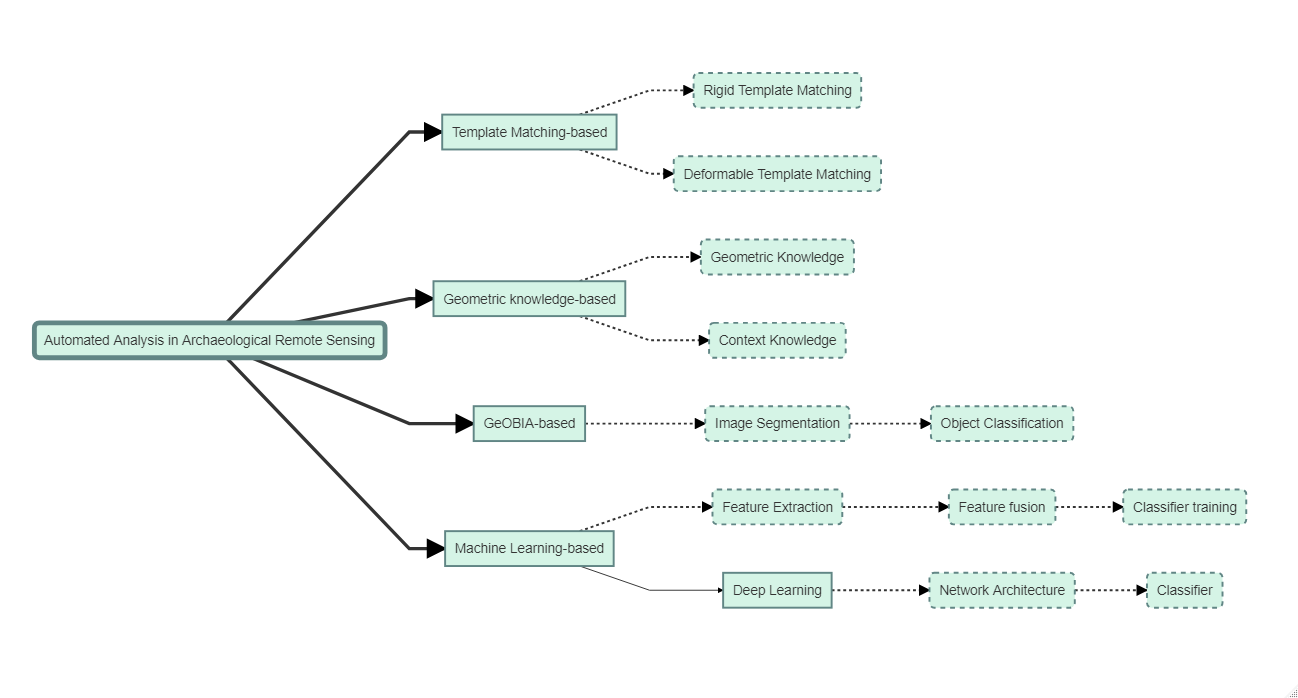
\includegraphics[width=0.5\linewidth,height=0.5\textheight]{C:/Users/kelto/Documents/iSEGMound/analysis/figures/Figure_4}

\}

\caption{Taxonomy of Automated Analysis in Archaeological Remote Sensing, based on Cheng and Han 2016.}

(\#fig:Figure\_4)
\textbackslash end\{figure\}
The point ``Details of method'' (iv) explains the workflow of the study in a nutshell, if comprehensible. Point v, ``Variables/Morphometric parameters'' highlights the variables and or morphometric parameters used in the study. ``OOI'' (vi) are the objects investigated. The point ``Scale'' (vii) implies the geographical range of the study, if it was applied to a broader region than the area on which the method was developed. The last two points (``Software'' - viii, and ``Access'' - ix) investigated give us hints about the accessibility of the dataset and the code. Especially in earlier studies, information about the software used is not mentioned and sometimes can only be guessed. In the case of ``Access'', apart from the information about accessible data and code it was also documented if there is a workflow (a comprehensible sequence of the steps of the workflow) or a flowchart (a very generalized workflow without clear steps) or if any of the equations used was published and or explained. It was also documented if any supplementary information or document was attached to the study which can guide to a better understanding for a possible reproduction of the study. Although all these points have been investigated, for practical reasons mainly the points (ii) RS (Remote Sensing) data, (iii) Method/s, (iv) Detail of method/s, (v) Variables/morphometric parameters, (vi) OoI/Object(s) of Interest, (viii) Software and (ix) Access is going to be elaborated in depth in this and the next chapter.

It is essential to discuss the basic traits of the used methods (iii) in short, concentrating on their application in Archaeological Remote Sensing. It has to be stressed, that still no semantic lingua franca (between Archaeological Remote Sensing and Computer Vision and Remote Sensing Methods) exists when talking about automated methods in Archaeological Remote Sensing, thus methods are addressed in different ways (or most commonly in a very simplified way) and it is not always possible to determine which exact method has been utilised (recently it is improving, but it depends where the authors put the focus of their work). First, when shortly discussing the basic traits of the methods and their use in Archaeological Remote Sensing, it is only focussed on the use of the different methods (what is used, where and when) since 2006, when tell mounds were first investigated using automated analysis methods. In the second part of this chapter the way of their use is investigated and analysed how the methods are used.

\textbf{\emph{Template Matching-based methods}} utilize a template of the Object of Interest to be detected, which is then statistically matched to the input image. Two general directions can be distinguished: Rigid Template Matching, which requires a precise template which gets problematic when it comes to intra-class shape and size variations. Deformable Template Matching on the other hand can handle either free-form deformable templates or parametric deformable templates. (Cheng and Han 2016, 13-14).
In the literature investigated Template Matching was used seven times for the detection of burial mounds, mound shell rings and tell mounds (De Boer 2007, Kramer 2015, Trier et al.~2015, Davis et al.~2018, Raun 2019, Davis et al.~2019, GholamReza and Malian 2021). Apart from Kramer 2015, Rigid Template Matching was preferred (Table 1). Template Matching itself is a method which is being revisited from time to time (Figure 5).

\begin{verbatim}
## [1] "Year"   "Method" "Freq"
\end{verbatim}

\textbackslash begin\{figure\}

\{\centering \includegraphics[width=0.75\linewidth,height=0.75\textheight]{Index_files/figure-latex/Figure_5-1}

\}

\caption{The Objects of Interests investigated by year between 2006 and 2021.}

(\#fig:Figure\_5)
\textbackslash end\{figure\}
\textbf{\emph{Geometric knowledge-based analysis}} works with specialized solutions for specific problems, applying rules based and established on knowledge of the regions of interest and it's context. It uses either encoded prior geometric knowledge of the generic specificity of the Object of Interest and then e.g.~applies hand-crafted mathematical morphometry rules for object extraction (morphometric derivatives such as Slope, Aspect, Curvature, Local Relief Model, vegetation indices etc.). Context knowledge based analysis uses knowledge about the relationship of the Object of Interest and the area it should be separated from (e.g.~filters, textural analysis) (Cheng and Han 2016, 15). In the case of Automated Archeological Remote Sensing the two Geometric knowledge-based analysis approaches are often used in combination and form the data preparation step (Figure 6). Geometric knowledge based object analysis is only occasionally used per se as an automated analysis method for the detection of burial mounds, monumental earthworks and tell mounds: Riley 2009, Freeland et al.~2016, Rom et al.~2020. (Lately) it is only occasional, that Geometric knowledge-based object analysis is not used as data preparation method (De Boer 2007, Caspari et al.~2014, Trier et al.~2015, Raun 2019, Caspari and Crespo 2019, Kazimi et al.~2019a, Kazimi et al.~2019b). In some cases, Geometric knowledge based analysis is included in the future work (compare works by Kazimi et. al 2019 vs.~Kazimi et al.~2020)(Table 1.).

\begin{verbatim}
## [1] "Year"   "Method" "Freq"
\end{verbatim}

\textbackslash begin\{figure\}

\{\centering \includegraphics[width=0.75\linewidth,height=0.75\textheight]{Index_files/figure-latex/Figure_6-1}

\}

\caption{The use of Geometric knowledge-based methods distributed by year between 2006 and 2021.}

(\#fig:Figure\_6)
\textbackslash end\{figure\}
\textbf{\emph{Geographical Object-based Image Analysis (GeOBIA)}} dates back to the late 1970's (Blaschke et al.~2014), but it was only around 2000 that Object-based Images Analysis became widely used in Remote Sensing studies due to the availability of high resolution Satellite data. This induced a paradigm shift not only in Remote Sensing but generally in GI Science, hence its new name: GeOBIA (Hay and Castilla 2008). GeOBIA operates in two steps: images are divided into small segments, which are defined by the homogeneity of specific morphometric (shape, size, orientation), spectral, textural, context and neighborhood parameters (Hay -- Castilla 2008) and are then grouped together to meaningful homogeneous object candidates (the segmentation step), which are then classified by specific extracted object criteria in question (the feature extraction and classification step, Blaschke et al.~2014, 186, Cheng and Han 2016, 15, Hossain and Chen 2019, 115) or filtered by a rule-set. Various types of segmentation methods exist (as also their categorization: Blaschke 2010, Blaschke et al.~2014, Kumar et al.~2014). Lately Hossain and Chen 2019 investigated the different segmentation methods from a Remote Sensing point of view, but here only the two main Segmentation methods used in Automated Archaeological Remote Sensing studies are described: Watershed Segmentation (or Transformation) (Niculiță 2020a,b) and Multiresolution Segmentation (Kramer 2015, Sevara et al.~2016, Freeland et al.~2016, Davis et al.~2018, Davis et al.~2019, Meyer-Heß et al.~2019, Sărășan et al.~2020), the first being an Edge-Based Segmentation method, the latter a Region-Based Segmentation method. For an in-depth analysis see Hossain and Chen 2019.

\emph{Edge-Based Segmentation techniques} are `top-down' methods: first they locate edges in the image and then use contouring algorithms to close them. Edges are regarded as boundaries between objects where pixel properties are abruptly changing (Hossain and Chen 2019, 117). `Watershed Segmentation' (implemented in open source software e.g.~in SAGA or in the ForestTools package in R) simulates real-life flooding. It first transforms the image into a gradient (grey-scale), then identifies objects with clear segment boundaries, only to then create (fill) objects, for which it is also called a Region-Growing algorithm (Hossain and Chen 2019, 117, Table 1; Figure 7).

\textbackslash begin\{figure\}

\{\centering 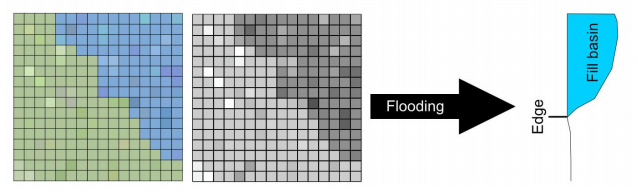
\includegraphics[width=8.86in]{C:/Users/kelto/Documents/iSEGMound/analysis/figures/Figure_7}

\}

\caption{Operating principle of ‘Watershed Segmentation’. Roffler 2020, 33.}

(\#fig:Figure\_7)
\textbackslash end\{figure\}
Region-Based Segmentation techniques start from the complete opposite: they begin with an initial segmentation of the whole image (thus also called `bottom-up methods') based on a specific rule-set. Regions are generated in two completely different ways: either by splitting the image into homogeneous regions based on inhomogeneity (region-splitting and then merging) or by region-growing from a so-called seed-region based on homogeneity (region-growing and then merging, Hossain and Chen 2019, 119). `Multiresolution Segmentation' (Baatz and Schäpe 2000, for which mainly eCognition is used in Automated Archaeological Remote Sensing) is a region-merging hierarchical segmentation method which starts with one pixel (seed) and applies pairwise merging of segments to build up hierarchical levels. The merging -- or clustering (using local rule sets) is repeated (on multiple levels), until an object is recognized (Hossain and Chen 2019, 119, Roffler 2020, 33-34; Figure 8).

\textbackslash begin\{figure\}

\{\centering 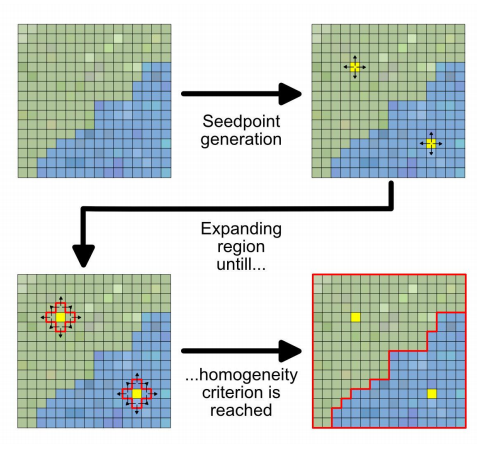
\includegraphics[width=0.75\linewidth,height=0.75\textheight]{C:/Users/kelto/Documents/iSEGMound/analysis/figures/Figure_8}

\}

\caption{Operating principle of ‘Region Growing Segmentation’. Roffler 2020, 34.}

(\#fig:Figure\_8)
\textbackslash end\{figure\}

With regard to (Automated) Archaeological Remote Sensing, GeOBIA is sometimes also called archaeOBIA (Lamotte and Masson 2016), which points to the fact, that (Automated) Archaeological Remote Sensing is in need of a completely different semantic ontology and rule sets than which is needed for customary GeOBIA methods used in Remote Sensing. Still recently the challenge in Remote Sensing has been to define segmentation parameters/rule sets which can be transferred to other images (Cheng and Han 2015, 16) -- something archeOBIA is also struggling with (see Table 1; note the different variables used in the different studies).
Burial mounds, monumental earthworks and mound shell rings have been investigated using GeOBIA methods nine times since 2015 (Figure 9). Apart from one case (Niculiță 2020: Watershed Segmentation, carried out with SAGA in R), Multiresolution Segmentation was applied (Table 1), almost exclusively using eCognition, (former Definiens), a software developed for and with the evolution of GeOBIA and thus is generally considered ``the software'' for GeOBIA (Blaschke 2010, Fig 4, Hossain and Chen 2019, Fig 1.), which is clearly reflected in this survey.

\begin{verbatim}
## [1] "Year"   "Method" "Freq"
\end{verbatim}

\textbackslash begin\{figure\}

\{\centering \includegraphics[width=0.75\linewidth,height=0.75\textheight]{Index_files/figure-latex/Figure_9-1}

\}

\caption{The use of GeOBIA methods distributed by year between 2006 and 2021.}

(\#fig:Figure\_9)
\textbackslash end\{figure\}
\textbf{\emph{Machine Learning-based methods}} are considered a subfield of Artificial Intelligence. Machine learning automates statistical methods to learn from input data either supervised, unsupervised or semi-supervised. Automated Archaeological Remote Sensing mainly utilizes supervised methods.
\emph{Pixel-based Image Analysis}, an image classification method, has been developed in the early 1970s for the digital analysis of Landsat Multispectral Scanner Systems (Phiri and Morgenroth 2017, 9) and is (still) widely distributed in Remote Sensing research, especially in land-use and land-cover classification. In contrast to GeOBIA, Pixel-based Image Analysis approaches an image on pixel basis, which are classified into different categories based on the information they carry (usually one variable). Given that the second step of GeOBIA can be a classification of the segmented image using variables of the image-objects best describing the Objects of Interest, GeOBIA is sometimes also seen as a form of Machine Learning (Davis 2018, 1).
Random forest classifiers are supervised learning algorithms which consist of an ensemble of decision trees. Each (unrelated) decision tree is trained using a random subset of the training data. Each of these trees will give a prediction for a datapoint. Then, the prediction of all decision trees is averaged by a majority vote to a final prediction (Figure 9). The independence of the different decision trees increases the accuracy of the prediction and also eliminates problems that can be caused by outliers in the dataset and works also well with small datasets, because of the facts just explained. These effects can be enhanced by resampling techniques and parameter tuning (Kuhn and Johnson 2016).

\textbackslash begin\{figure\}

\{\centering 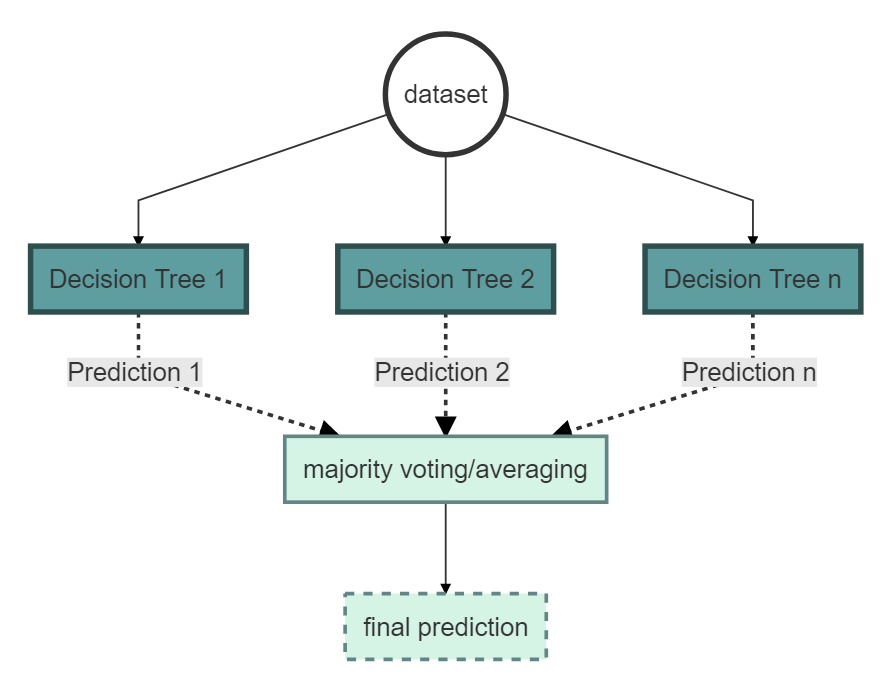
\includegraphics[width=0.5\linewidth,height=0.5\textheight]{C:/Users/kelto/Documents/iSEGMound/analysis/figures/Figure_10}

\}

\caption{Schematized modus operandi of the Random Forest algorithm.}

(\#fig:Figure\_10)
\textbackslash end\{figure\}
Regarding the automated detection of burial mounds and similar structures, Pixel-based classification was the first method used in 2006 and has been more or less revisited since (Figure 11). When looking closely at the specific algorithms used, it is not surprising why the Random Forest algorithm was exploited in most Pixel-based Image Analysis studies (Menze et al.~2006, 2007, Menze and Ur 2007, 2012, 2013, Kramer 2015, Guyot et al.~2018, Orengo et al.~2020, Niculiță 2020, Davis et al.~2021) and Mahalanobis Distance (Trier et al.~2015, Severa et al.~2016) and Support Vector Machine Classifiers (Caspari and Crespo 2019) in less.

\begin{verbatim}
## [1] "Year"   "Method" "Freq"
\end{verbatim}

\textbackslash begin\{figure\}

\{\centering \includegraphics[width=0.75\linewidth,height=0.75\textheight]{Index_files/figure-latex/Figure_11-1}

\}

\caption{The use of Pixel-based Image Analysis methods distributed by year between 2006 and 2021.}

(\#fig:Figure\_11)
\textbackslash end\{figure\}
It was already suggested that with the development of remote sensing sensors and resulting new, higher resolution datasets the need for new analysis methods is constantly stimulated. Starting with pixel-wise analysis and followed by the object-level addressing of remote sensing imagery, lately an even bigger semantic step was taken: the analysis on the scene-level, which can be seen as the next paradigm shift (Cheng and Han 2016, Cheng et al.~2020, 2, Fig. 2). The complex semantic structures of very high resolution images are addressed by \emph{Deep Learning}, which is also a sub-field of Machine Learning. In contrast to Pixel- and Object-based Image Analysis, Deep Learning Algorithms consist of multiple stacked hierarchical layers (network architectures) which can handle complexity and abstraction.
In the case of the identification of burial mounds and mound like structures Deep Learning is only in use since 2019 (Figure 12).

\begin{verbatim}
## [1] "Year"   "Method" "Freq"
\end{verbatim}

\textbackslash begin\{figure\}

\{\centering \includegraphics[width=0.75\linewidth,height=0.75\textheight]{Index_files/figure-latex/Figure_12-1}

\}

\caption{The use of Deep Learning methods distributed by year between 2006 and 2021.}

(\#fig:Figure\_12)
\textbackslash end\{figure\}
To summarize the use of automated analysis methods to detect burial mounds and mound-like structures (Figure 13), it can be established that the first method used was Pixel-based Image analysis (Menze et al.~2006), followed by Template Matching (de Boer 2007). Geometric knowledge-based analysis was used as an autonomous method only by Riley 2009, Freeland et al.~2016, Rom et al.~2020, but as already concluded it is more often than not incorporated in workflows as data preparation method. GeOBIA was first used in 2015 and remained a very effective analysis method, until recently when Deep Learning became widespread (including Semantic and Instance Segmentation).

\textbackslash begin\{figure\}

\{\centering \includegraphics[width=0.75\linewidth,height=0.75\textheight]{Index_files/figure-latex/Figure_13-1}

\}

\caption{The use of different Image Analysis methods to detect mounds and mound-like objects distributed by year between 2006 and 2021. Note: this represents the number of methods used, not the number of studies.}

(\#fig:Figure\_13)
\textbackslash end\{figure\}
Several studies compare different analysis methods or combine them. Freeland et al.~2016 and Davis et al.~2019 compare Geometric-knowledge-based analysis (iMound/Inverse Stochastic Depression Analysis) to GeOBIA, with success (this is also reflected in the fact that the original algorithm iMound by Freeland at al.~2016 was reused by Davis et al.~2019 and Rom et al.~2020). Template Matching has been compared to GeOBIA (Kramer 2015, Davis et al.~2019: including Geometric knowledge-based method) and Pixel-based Image Analysis to GeOBIA (Sevara et al.~2016) and to Deep Learning (Caspari and Crespo 2019).

Although LiDAR data has been available for some time (see De Boer 2007, Riley 2009), it was only after 2010 that it made its way into everyday archaeological research, including various visualization methods (as Geometric knowledge-based analysis and data preparation method), making LiDAR visualisations a self-evident step for any archaeological project using ALS data (see also Kokalj and Hesse 2017). It is mainly from 2015, when ALS data started to dominate and revolutionize Automated Analysis methods in Archaeological Remote Sensing and provoking new approaches, such as GeOBIA (Figure 14). Since the diffusion of LiDAR data, Satellite Imagery is mainly used in large-scale studies (Caspari and Crespo 2019, Orengo et al.~2020). Studies which require high resolution data and utilize LiDAR quickly shifted to Deep Learning solutions. Simultaneously also UAV data finds its way into the general data repertoire of Automated Archaeological Analysis (Sărășan et al 2020).

\textbackslash begin\{figure\}

\{\centering \includegraphics[width=0.75\linewidth,height=0.75\textheight]{Index_files/figure-latex/Figure_14-1}

\}

\caption{The use of different data types used to detect mounds and mound-like objects distributed by year between 2006 and 2021.}

(\#fig:Figure\_14)
\textbackslash end\{figure\}
When taking the points `Software' and `Access' into account, it has to be expressed that it is only a recent phenomenon that software and computation details have to be disclosed when publishing a study. Even though lately many journals require data and code availability statements, only a few studies provide openly accessible code and data: Orengo et al.~2020, and Niculiță 2020. In the first case the data and the code are available using Google Earth Engine. In the latter case, the regulations of the local Cultural Heritage Management authorities require a signed form through the author of the study to be able to use the DEM on which the study was based on - nonetheless it can be accessed. Although with restrictions.
Inspecting the information about the methodology details of the studies, nine cases have been identified (Figure 15): from not available (n/a) to workflow \& code \& data, many constellations can be observed. In many cases the workflow was published, in some cases only a flowchart. In this thesis as a workflow the clear explanation of the methodology in a chart form is defined (with a big probability of reproducibility if the observer knew the exact tools and software used or if those were made clear). As a flowchart on the other hand, a part of a workflow or a very schematized workflow was identified where only the main steps were arranged in chart form, thus making it impossible to trace back the specific steps and to reproduce the workflow or any part of it. Thus the only reproducible study, which published a really detailed workflow, the code and made the dataset - although restricted by certain rules - available is Niculiță 2020.

\textbackslash begin\{figure\}

\{\centering \includegraphics{Index_files/figure-latex/Figure_15-1}

\}

\caption{Access to any parts of  studies used to detect mounds and mound-like objects distributed by year between 2006 and 2021.}

(\#fig:Figure\_15)
\textbackslash end\{figure\}
As already noted, eCognition is considered ``the'' software for GeOBIA (Hossain - Chen 2019, 122) thus it is evident that many will choose this simpler solution. At the same time, it must be emphasised that the first analyses were carried out in R (Menze et al.~2006, Menze et al.~2007, Menze and Ur 2007), i.e.~with open source software.. Using proprietary software not only marginalises researchers and institutions who/which can't afford rather expensive software, but it is also hard to comprehend the exact algorithm behind the software, and to understand to be able to apply it in another domain. It is also important to understand why certain tools or algorithms worked or did not work? This can only be done by creating reproducible workflows with open source software. In 2019 and 2020 more than 60\% of the studies were conducted with FOSS (Free and Open Source Software) software. This number is only increasing (Figure 16).

\textbackslash begin\{figure\}

\{\centering \includegraphics{Index_files/figure-latex/Figure_16-1}

\}

\caption{Software types of studies used to detect mounds and mound-like objects distributed by year between 2006 and 2021.}

(\#fig:Figure\_16)
\textbackslash end\{figure\}
This survey served the purpose to elaborate the development of Automated Analysis in Archaeological Remote Sensing, mainly with regard to the applied methods, the used software and access to information about the workflow. The aim was to show how little reproducible research has been published with regard to automated analyses and how much there is to be done in the future. Also, automated analysis in Archaeological Remote Sensing is being carried out on different scales with different algorithms, specialized to different research questions in mainly research contexts. This is also a reason why many critical voices see automated analysis methods as pastimes and not really something operational (see many AARGnews Editorials). To give way for the next chapter we can conclude that the results of automated analyses are compelling, but many studies start basically from the beginning, because when research is published without accompanying software, workflow, data and documented steps, it is a challenge and time consuming to understand, verify, expand and eventually surpass that research (Marwick 2017, 425). This is one reason why many research projects start from the beginning, with a new idea instead of building on the previous knowledge. Another point is that automated analysis methods in Archaeological Remote Sensing are still in their infancy (Opitz and Herrmann 2018, 30) and best practices have not yet been established. Nonetheless it has to be stated that automated analysis itself is not a goal, but a method, a means to an end to further research and thus reproducible or even replicable best practices would help shift the focus on further development of methods than on continuous recommencements.

Chapter II discussed the use of automated analysis methods in Archaeological Remote Sensing for the detection of burial mounds and structurally similar archaeological objects. It was demonstrated that only 2 out of 31 studies have disclosed workflow, code and data and are thus reproducible (see chapter III for explanation). As a reproducible study in the R environment Niculiță 2020 can be taken as the best example. It was also noted that even without the availability of code, there are workflows which are illustrated and also explained clearly enough that they can be reproduced, which on the other hand can take some time but is still possible to do when having enough experience with spatial tools.
On this basis it was decided that the Geometric knowledge-based workflow `iMound' (established by Freeland at al.~2016 and reused by Davis et al.~2019 and Rom et al.~2020) is going to be utilized in R to detect burial mounds in LiDAR data in this Master's thesis to create a reproducible workflow. During the implementation of the workflow it became clear that on the basis of the geomorphometry of the Train Area it was necessary to include another method to be able to effectively detect burial mounds (this is discussed in depth in Chapter IV). Thus, in addition to `iMound' also the reproducible workflow of Niculiță 2020, thus a GeOBIA method was used in this Master's thesis.

\newpage

\hypertarget{the-necessity-of-a-paradigm-shift-in-archaeological-remote-sensing-practice-by-means-of-tool-driven-automated-analysis}{%
\section{The Necessity of a Paradigm Shift in Archaeological Remote Sensing practice by means of Tool-driven Automated Analysis}\label{the-necessity-of-a-paradigm-shift-in-archaeological-remote-sensing-practice-by-means-of-tool-driven-automated-analysis}}

In Chapter II the arguments of reproducibility and replicability have been addressed regarding the accessibility of data, code and workflow of the investigated studies. It was demonstrated that only 2 out of 31 studies have disclosed all three elements and are reproducible. It is important to discuss the exact definition of both expressions. In this Master's thesis mainly the definitions of Marwick 2017 are followed.
Reproducibility means that code and workflow of an analysis reproduces all results and figures in the respective publication from its original raw data. Replicability stands for the replication of the workflow (from data collection to data analysis) onto a new dataset. It was mentioned in the introduction that optimal reproducible open science would incorporate version controlled open code, clear workflows and open datasets or at least training datasets.

So then, how is the best way to implement and guarantee reproducibility? Marwick 2017 outlined four general principles of reproducible research:
i) Data and code provenance, sharing and archiving (analogue to artifact provenience)
ii) Scripted analyses (for reproducibility and ideally replicability)
iii) Version control (transparency of decision points of any research and possibility of collaboration)
iv) Self-contained computational environments (sharing the computational environment of the analysis for replicability).

Pushing forward along this road, Marwick et al.~2018 propose R-packages as research compendia to organize transparent and reproducible research to approach the general principles laid out in 2017. Research compendia should organize files according to conventions: separate data, method and output (the latter being disposable because they can be reproduced) and define which exact computational environment was used for the analysis. Building an R package around a research project automatically forces one to keep the guidelines and conventions of package building which also provides quality control mechanisms.
Research compendia come in many forms and complexities, as Marwick et al.~2018 discusses. The author of this Master's thesis experimented with a basic form of reproducible research compendium when analysing the finds of an Iron Age cemetery in Hungary using multivariate statistical analysis (Schneider 2020). The work was done basically in an R project with a fixed project structure which was uploaded in a github repository (\url{https://github.com/keltoskytoi/Multivariate_Statistics_Szentloerinc}). The repository contains an .Rproj file with the settings for the project, a folder called DATA for the raw data to be analyzed and not to be changed during the study, two .R files with the code used for the analysis in the study, a README.md file with basic information of the paper, thus the title and where to get it. An earlier study and research compendium from 2015, but already in a very mature form by Ben Marwick already shows the many of the elements of an optimal research compendium (listed in Figure 12), organized as an R package with the published compendium on figshare for the study Clarkson et al.~2015 which is also completely replicable: \url{https://github.com/benmarwick/1989-excavation-report-Madjedbebe}; \url{https://figshare.com/articles/software/1989_excavation_report_Madjebebe/1297059}
A recent use of a research compendium is Schmid 2019 with the compendium published at OSF. This study is also completely replicable:
(\url{https://github.com/nevrome/cultrans.bronzeageburials.article2019}, \url{https://osf.io/b6np2/})
Based on the reproducibility of these studies and on the personal experience and motivation mentioned above, it was decided to create a research compendium for the Master's thesis.

The optimal outline for a complex research compendium in an R environment is reproduced from Marwick et al.~2018, Figure 4:

\textbackslash begin\{figure\}

\{\centering 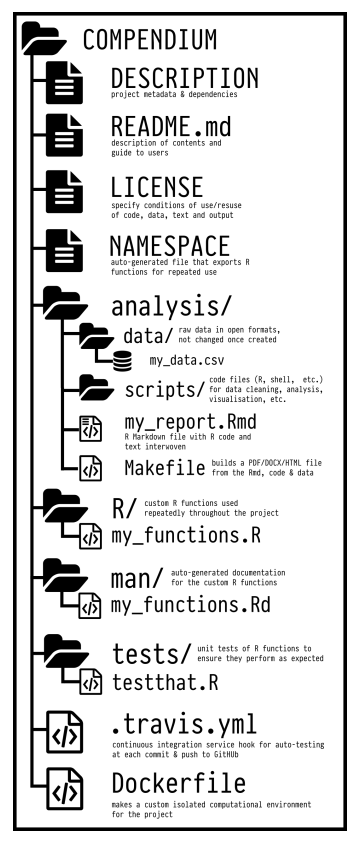
\includegraphics[width=0.5\linewidth,height=0.5\textheight]{C:/Users/kelto/Documents/iSEGMound/analysis/figures/Figure_17}

\}

\caption{Figure 17. Schematized modus operandi of the Random Forest algorithm.}

(\#fig:Figure\_17)
\textbackslash end\{figure\}

This optimal research compendium outline is implemented in the R package rrtools (`reproducible research tools', \url{https://github.com/benmarwick/rrtools}) by Ben Marwick, which helps to write reproducible research papers, setting up the structure propagated in Marwick et al 2018. Although this Master's thesis cannot give place to all of these desired steps and tools, it shall provide a reproducible workflow for burial mound detection using R.

R is an open-source, open-access statistical scripting language which can be used either through the command line or it's GUI, R Studio. It has been used in several scientific domains, and lately it is one of the most commonly used scripting languages in Archaeological Sciences (Schmidt and Marwick 2020, 18). The advantages of scripting languages support the four general principles of reproducible research of Marwick 2017 (see above) which are embodied in an optimal research compendium. The use of scripting languages (can) facilitate the use of Automated Analysis methods in Archaeological Remote Sensing, by offering a clear and logical semantic syntax, delivering a (shared diachronic semantic) ontological consistency throughout the research project and for future use.

Schmidt and Marwick 2020 -- after discussing idea- and tool-driven revolutions in science -- debate the role of tools in paradigm-shifts in Archaeology. Archaeology is in a paradoxical situation: for one it is mainly an idea-driven discipline, but it has seen multiple tool-driven paradigm shifts (e.g.~with Clarke's Analytical Archaeology and the development of Computational Archaeology). Computational Archaeology, Archaeological Remote Sensing and Remote Sensing itself are disciplines where change is mainly tool-driven, as we can see based on Chapter 2, which analysed 31 papers. But tools also ignite ideas, so there is no clear distinction, more a self-induction.

Before going to the next step, the concept of ``tool-driven'' has to be investigated more thoroughly. Schmidt and Marwick 2020 borrow the concept from Galison 1997, who elaborated on a tool-driven change in particle physics in the twentieth century, meaning tools like digital devices (for instance computers in the case of Archaeology). They see R (or similar open source programming languages) as one projection of a tool-driven revolution, including sharing reproducible and replicable code (Schmidt and Marwick 2020, 19). In my opinion we have to go further - the concept of tool-driven should become more mundane and tangible: automated analysis in Archaeological Remote Sensing has to become tool-driven in order to present a robust scientific practice for Archaeology, which means that reproducible workflows have to be created to do specific tasks, such as feature extraction, segmentation, which can then be developed further and be learned from. Automated analysis in Archaeological Remote Sensing should embrace tool-driven reproducible research to the fullest to make it possible to learn from each other and to build upon the experience of each other to develop ideas further.

One important issue still needs to be addressed. Lately it has been stressed (Strupler 2021) that not all openly published data are comparable: only because the raw data, especially if they are older projects which do not comply yet with the Berlin Declaration on Open Access to Knowledge in the Social Sciences and Humanities, is openly published and the exact methods are known, it does not automatically grant reproducibility (Strupler 2021, 2.). This emphasizes, that not only new data, reproducible workflows and best practices need to be created and published according to guidelines, but also legacy data from on-going, long-term excavations should be revised and curated and updated, to fit the FAIR principles `Findability', `Accessibility', `Interoperability', and `Reuse' (Haas and van Leusen 2020). It is clearly a problematic issue in this case, because often the authors might not be retractable. Thus reproduction of previous studies is a good way to correct, curate and update these datasets and the code and data is perfect for learning and teaching workflows but also to learn how to deal with possible errors (Strupler 2021, 15). It has to be pointed out that it cannot be expected to have complete consistency between a dataset processed in the original study using a GIS platform and then replicated using a scripting language. When using software other than a scripting language (where optimally all steps taken are documented), there are often steps one does not document or forge. An error in a dataset or analysis is a different matter and complicates reproducibility but should not have a negative connotation and should not be seen as a failure in the archaeological scientific community but treated with `full disclosure', as a learning effect on how to make datasets and analysis better. The valid point is raised, that when publishing datasets and analysis there should be a responsible person to turn to (Strupler 2021, 16-17). This is even true when e.g.~in a project the data is collected by a different person than the one who will do the analysis. Often crucial information is already missing when doing the analysis in the first place and this also needs to be disclosed clearly in the analysis (metadata in any form suitable for the project) and is not to be left out. In the case of datasets made available in an online repository, the owner of the repository or provider (uploader) of the dataset seems to be the logical person to make responsible if not disclosed otherwise. This can be of course problematic with legacy datasets.

This comes together with the development of best practices and publishing datasets with workflows as mentioned before and fits perfectly in the wider picture of the Reproducible Research Culture (Nakoinz 2021, 63). Reanalysis studies are the perfect means to test reproducibility and the quality of data and metadata (as seen above).
Like Quantitative Archaeology, also Automated Archaeological Remote Sensing needs a paradigm shift from a closed and restrictive to a sustainable Open Science.

\newpage

\hypertarget{applied-mound-detection}{%
\section{Applied Mound Detection}\label{applied-mound-detection}}

In certain instances it was decided to use screenshot to be able make points clearer. It was planned to use mapview::mapview, but it does not knit nicely when exported as a PDF.

\newpage

\hypertarget{results-of-the-isegmound-workflow}{%
\section{Results of the iSEGMound Workflow}\label{results-of-the-isegmound-workflow}}

In this Master's thesis two data preparation methods (using a plain DTM vs.~a Multi-Scale Topographic Index, as described an explained in Chapter 4) and two segmentation methods (Watershed and Region Growing, as described in Chapter 2 and explained in Chapter 4) were examined, applied and compared, resulting in four workflows. The basic settings and the exact structure and process for the four workflows were tested and debugged on the Train DTM (one 1x1 km tile) and then applied and to the Train Area (five 1x1 km tile) to understand the relationship between the size of the area of investigation and the variable settings of the respective algorithms. These settings were the adjusted and the most effective workflow was chosen (based on the Train Area). This was followed by the application of the selected workflow to the five Areas of Interests: AoI 1, AoI 2, AoI 3, AoI 4 and AoI 5.

First let's have inspect the chosen morphometric derivative, the Multi-Scale Topographic Index (later MSTPI), on the example of the Train DTM:

\textbackslash begin\{figure\}

\{\centering 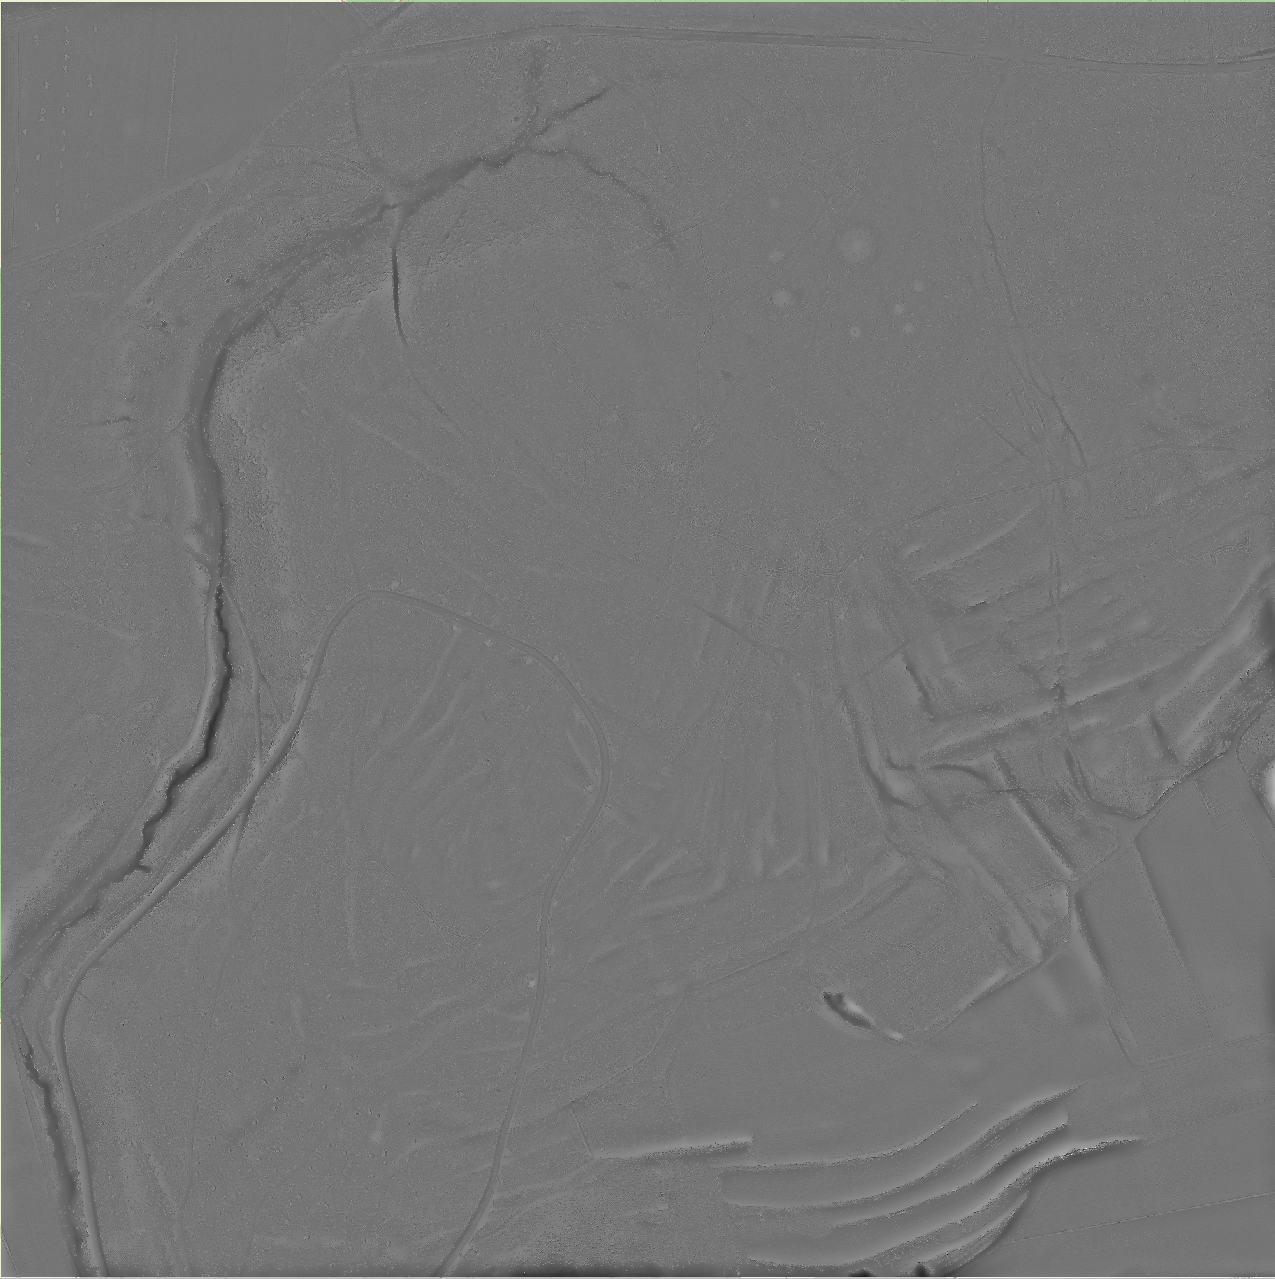
\includegraphics[width=1\linewidth,height=1\textheight]{C:/Users/kelto/Documents/iSEGMound/analysis/figures/Figure_67}

\}

\caption{Multi-Scale Topographic Index of the Train DTM, Scale 1:4450.}

(\#fig:Figure\_67)
\textbackslash end\{figure\}
As a reminder let's see where the burial mound groups Site ID 5 (black) and Site ID 35 (blue) are located in the Training DTM:

\textbackslash begin\{figure\}

\{\centering 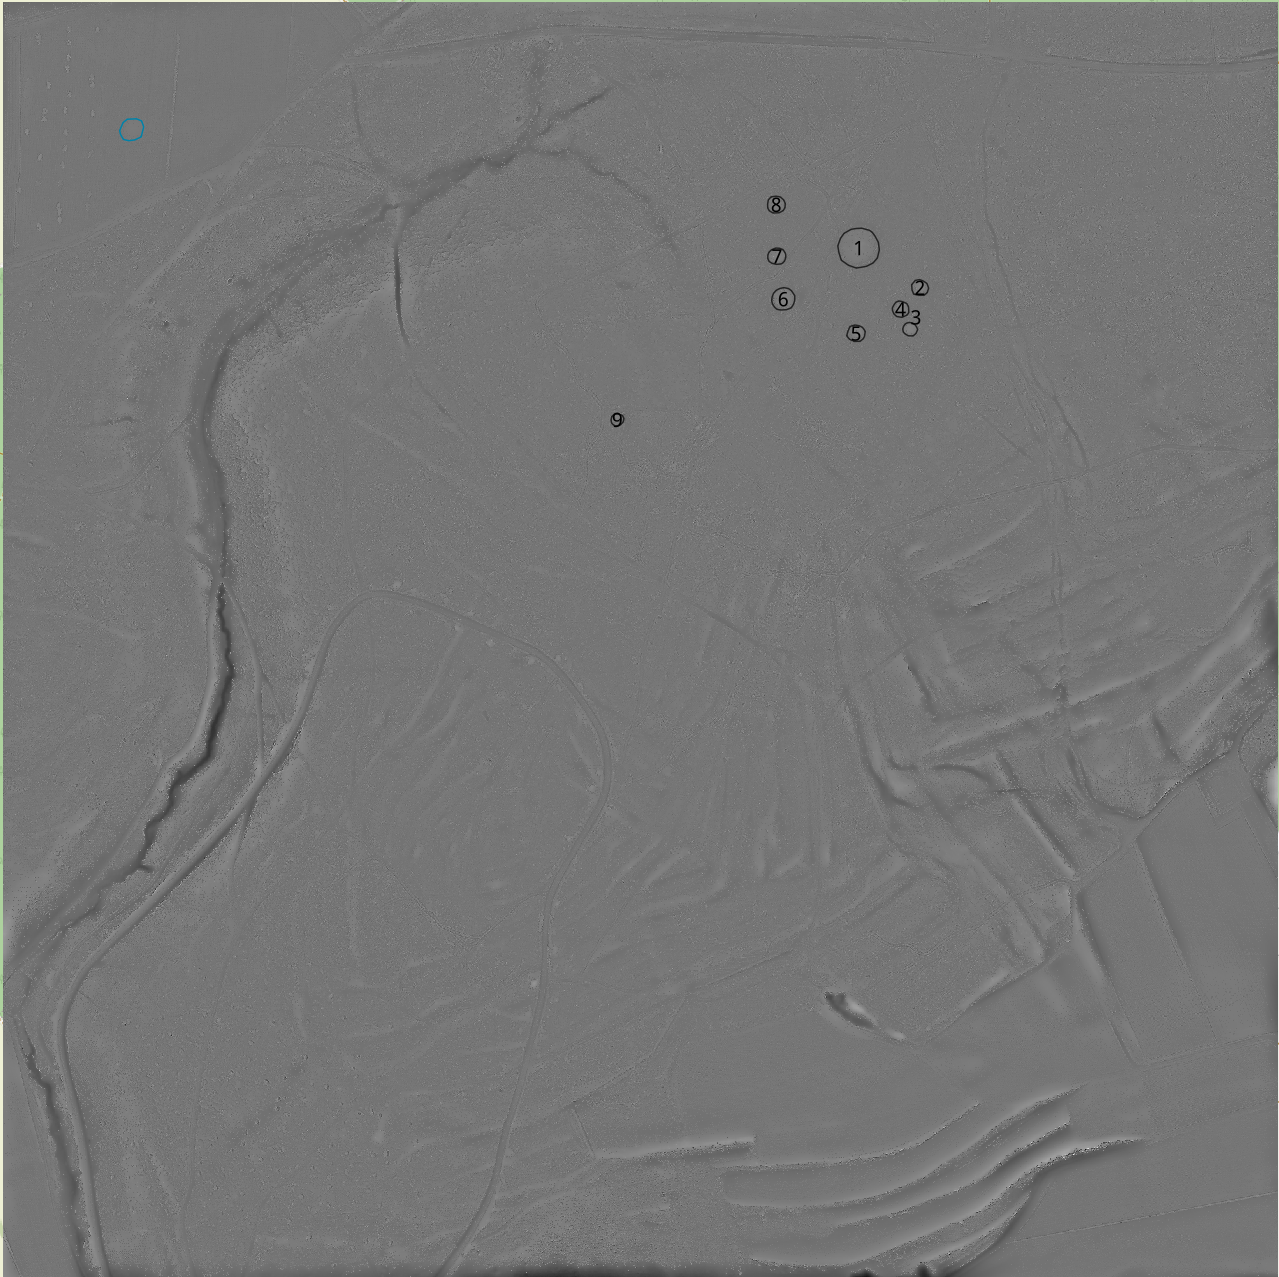
\includegraphics[width=0.5\linewidth,height=0.5\textheight]{C:/Users/kelto/Documents/iSEGMound/analysis/figures/Figure_68}

\}

\caption{Multi-Scale Topographic Index of the Train DTM with bruial mound groups Site ID 5 and 35. Scale 1:4450.}

(\#fig:Figure\_68)
\textbackslash end\{figure\}
We know from Dobiat et al.~1994, that Site ID 35 was identified as two mounds. As in Chapter 4 discussed, the mounds visible in Figure 68 were possible to be identified on ground.

\hypertarget{results-of-the-training-dtm}{%
\subsection{\texorpdfstring{\textbf{Results of the Training DTM}}{Results of the Training DTM}}\label{results-of-the-training-dtm}}

The workflows applied on the Training DTM are the following:
5a\_iSEG05\_WS, 5b\_iSEG05\_mtpi\_WS, 5c\_iSEG05\_RG, and 5d\_iSEG05\_mtpi\_RG.

Let's plot the results of the Training DTM by segmentation.
Left the Watershed Segmentation based on a DTM (iSEG05\_WS, orange segments) and on the SAGA MTPI (iSEG05\_mtpi\_WS, lilac segments). Right the Region Growing Segmentation based on a DTM (iSEG05\_RG, light blue) and on the SAGA MTPI (iSEG05\_mtpi\_RG, brown):

\textbackslash begin\{figure\}
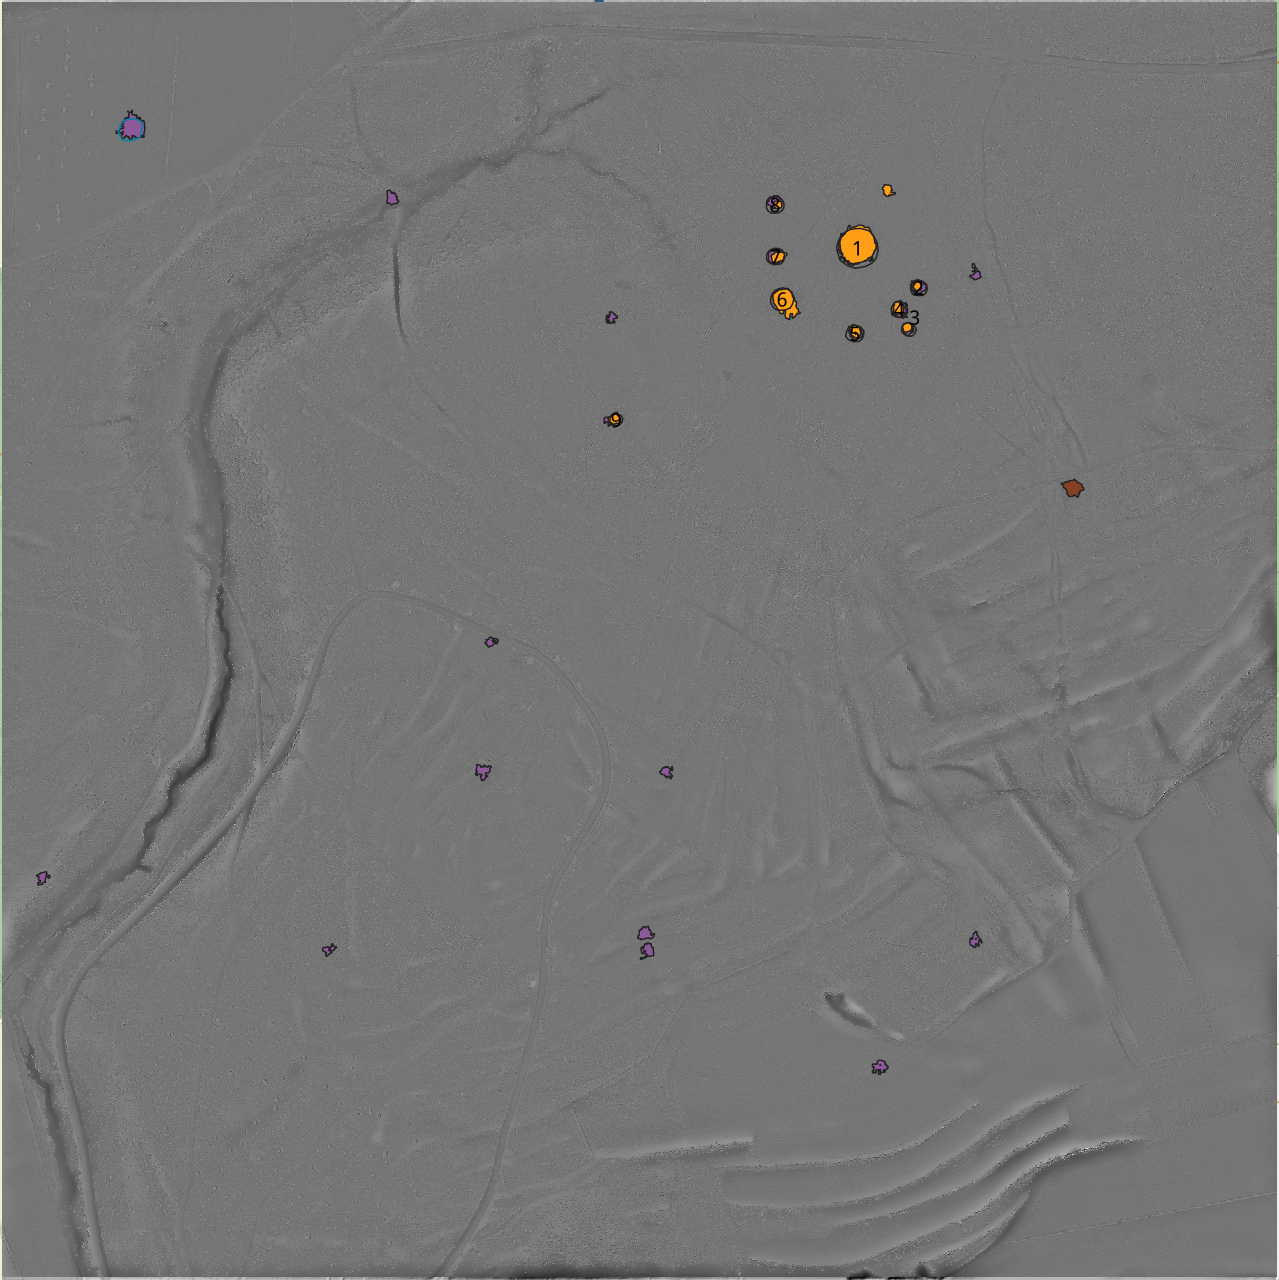
\includegraphics[width=0.5\linewidth,height=0.5\textheight]{C:/Users/kelto/Documents/iSEGMound/analysis/figures/Figure_69_1} 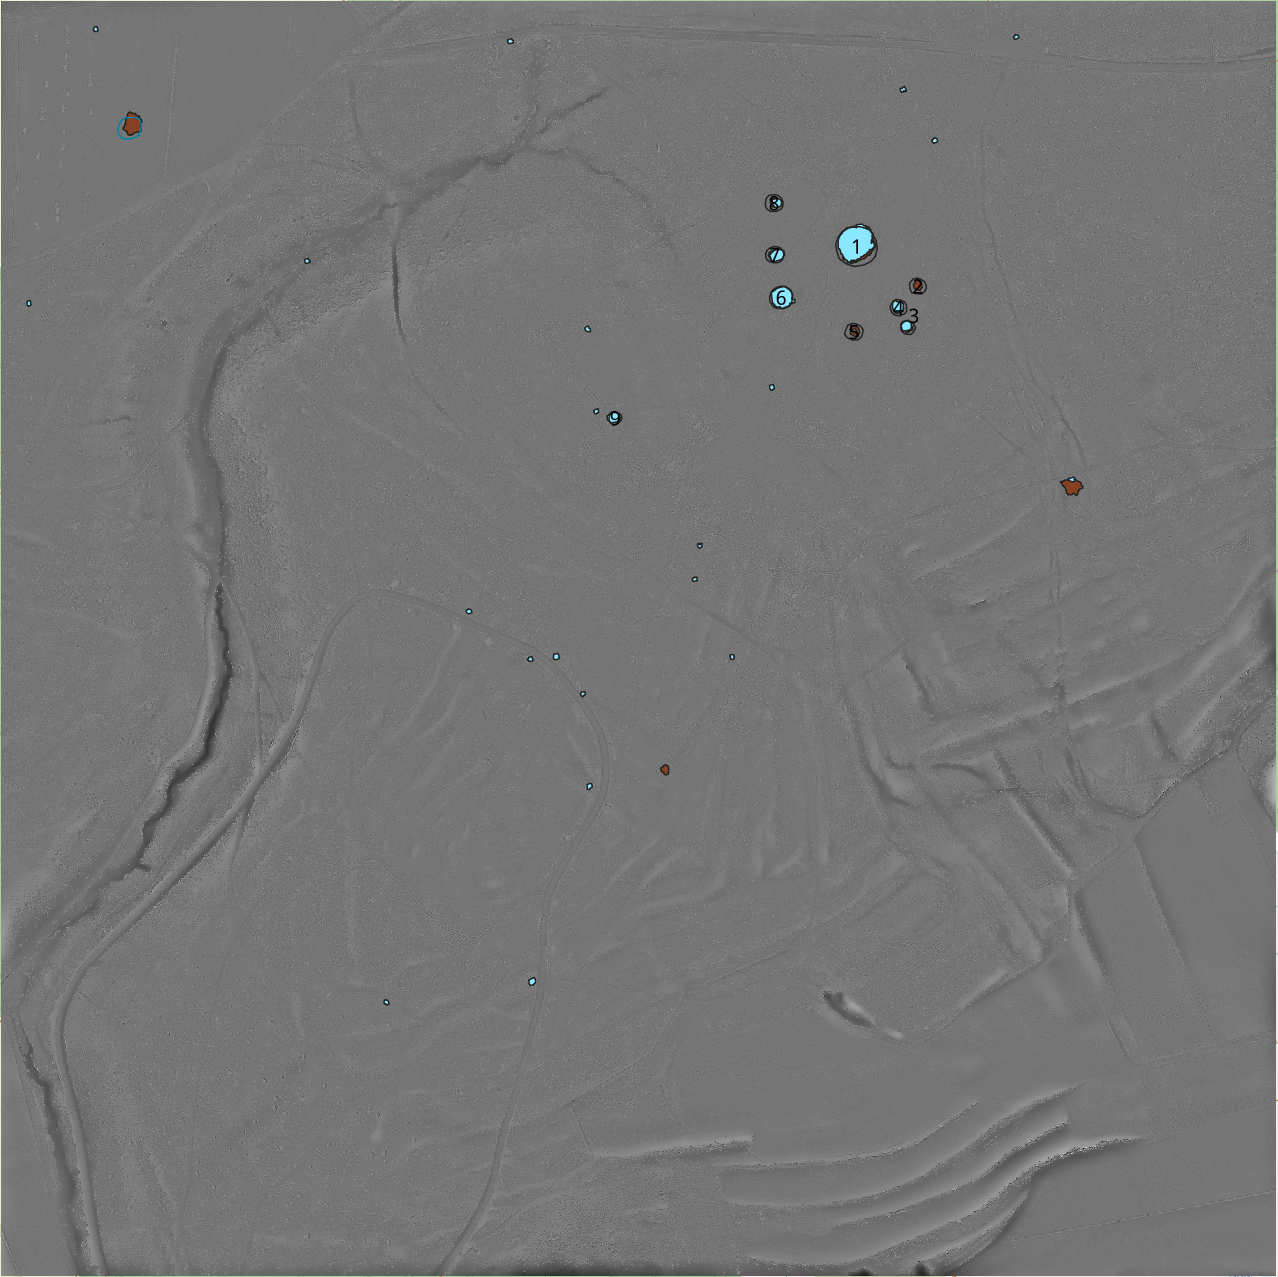
\includegraphics[width=0.5\linewidth,height=0.5\textheight]{C:/Users/kelto/Documents/iSEGMound/analysis/figures/Figure_69_2}

\caption{iSEG WS in orange and iSEG mtpi WS in lilac nect to iSEG RG in light blue and iSEG mtpi RG in brown, Scale 1:4450.}

(\#fig:Figure\_69)
\textbackslash end\{figure\}

The first thing that catches the eyes is that both segmentation methods were able to detect Site ID 35, using the SAGA MTPI. Thus it is already clear from this early step on, that in the case of these scarcely preserved burial mounds it is useful to work with morphometric derivatives. When comparing the two segmentation methods, it is apparent, that Watershed segmentation produces more segments than Region Growing.

\hypertarget{results-of-the-training-area}{%
\subsection{\texorpdfstring{\textbf{Results of the Training Area}}{Results of the Training Area}}\label{results-of-the-training-area}}

Before discussing the results of the segmentations, first let's inspect Site ID 7 and Site ID 14.

Site ID 7 is situated relatively near to the North of Site IDs 5 and 35. The group is constituted of 9 burials, roughly in an elongated line, counted from Southwest to Northeast. When inspecting the mounds, it can be seen that, similar to Site ID 5-9, these are also very near to the forestry commuting routes. Also they already show erosion (mound Site ID 7-5 to 9), mainly in road proximity. This situation has already worsened since 2009/2010, the collection date of the LiDAR data. This burial mound group is similarly preserved such as the average height of the mounds of Site ID 5.

Site ID 14 stretches a little further away to the South and consists of altogether 18 burials. This burial mound group spreads similarly elongated as Site ID 7, although a grouping can be made out in the center region of the group. What is striking about this group is, that many of the mounds - apart from mound 8, which is cut right at the middle - have been just missed or only slightly touched by service roads. The situation of burial mound Site ID 14-8 already indicated, that it is going to be hard to detect this mound properly, because it might be will be difficult to distinguish from the road which is cutting it.

\textbackslash begin\{figure\}
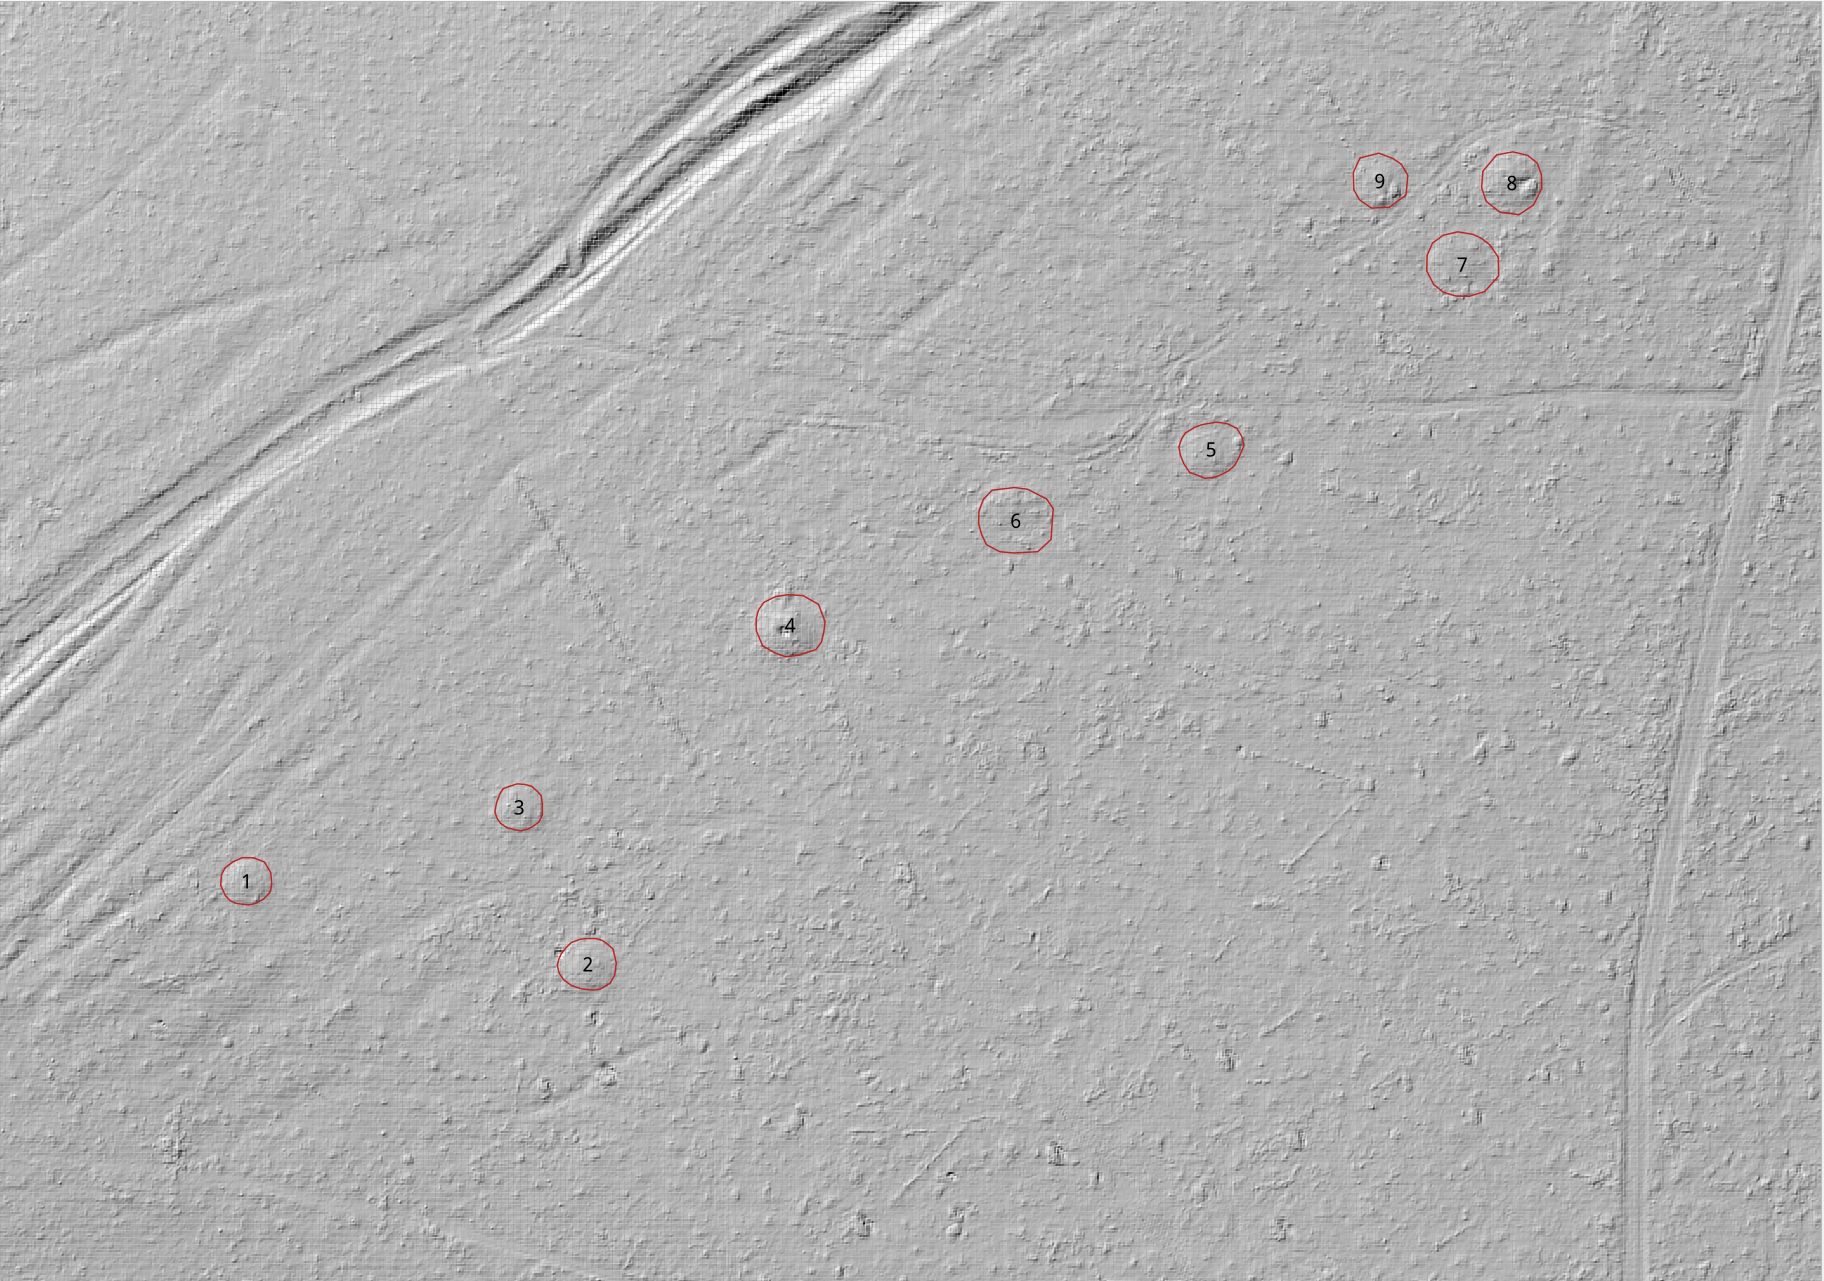
\includegraphics[width=0.5\linewidth,height=0.5\textheight]{C:/Users/kelto/Documents/iSEGMound/analysis/figures/Figure_70_1} 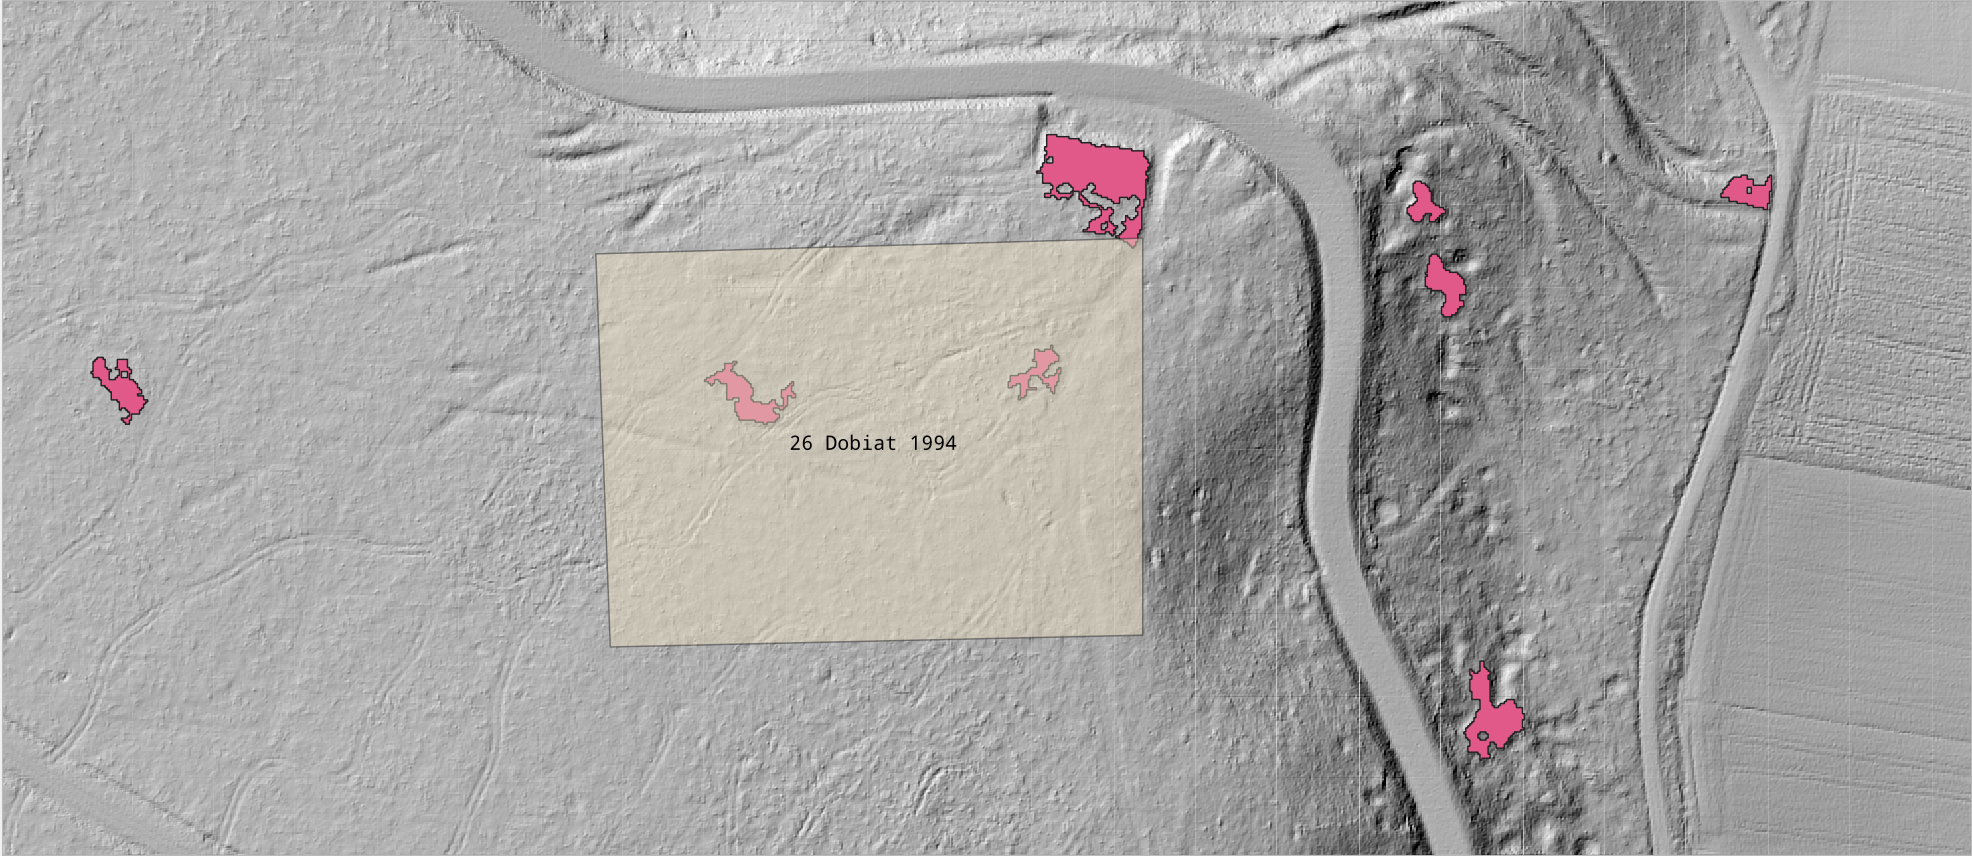
\includegraphics[width=0.5\linewidth,height=0.5\textheight]{C:/Users/kelto/Documents/iSEGMound/analysis/figures/Figure_70_2}

\caption{Site ID 7, consituted of 9 burial mounds and Site ID 14, constituted of 18 burial mounds on the DTM, Scale 1:1200 and 1:3100.}

(\#fig:Figure\_70)
\textbackslash end\{figure\}

The workflows applied on the Training Area are the following:
6a\_iSEG05\_WS\_ta, 6b\_iSEG05\_mtpi\_WS\_ta, 6c\_iSEG05\_RG\_ta, 6d\_iSEG05\_mtpi\_RG\_ta.

Because the Training Area is too big to really see details when plotting the whole, three plots are going to be displayed: one overview to understand the amount of segments and then the two areas containing burial mounds (Site IDs 5, 7 and 35 and Site ID 14) will be plotted next to each other to see the exact segmentation results.

Inspecting first the results of the Watershed Segmentation of the Training Area, iSEG05\_WS\_ta (pink segments) and iSEG05\_mtpi\_WS\_ta (teal segments) are plotted together. It is clearly visible from the overview, that the first impression of the Training DTM is reinforced: more segments are left over by using the SAGA MTPI, which fit to \emph{min} to \emph{max} descriptor range as the segments complying to the burial mound mask. This means on the other hand of course more segments to check, but also more possibility to find previously not known mounds. This will be investigated in the Discussion.

\textbackslash begin\{figure\}

\{\centering 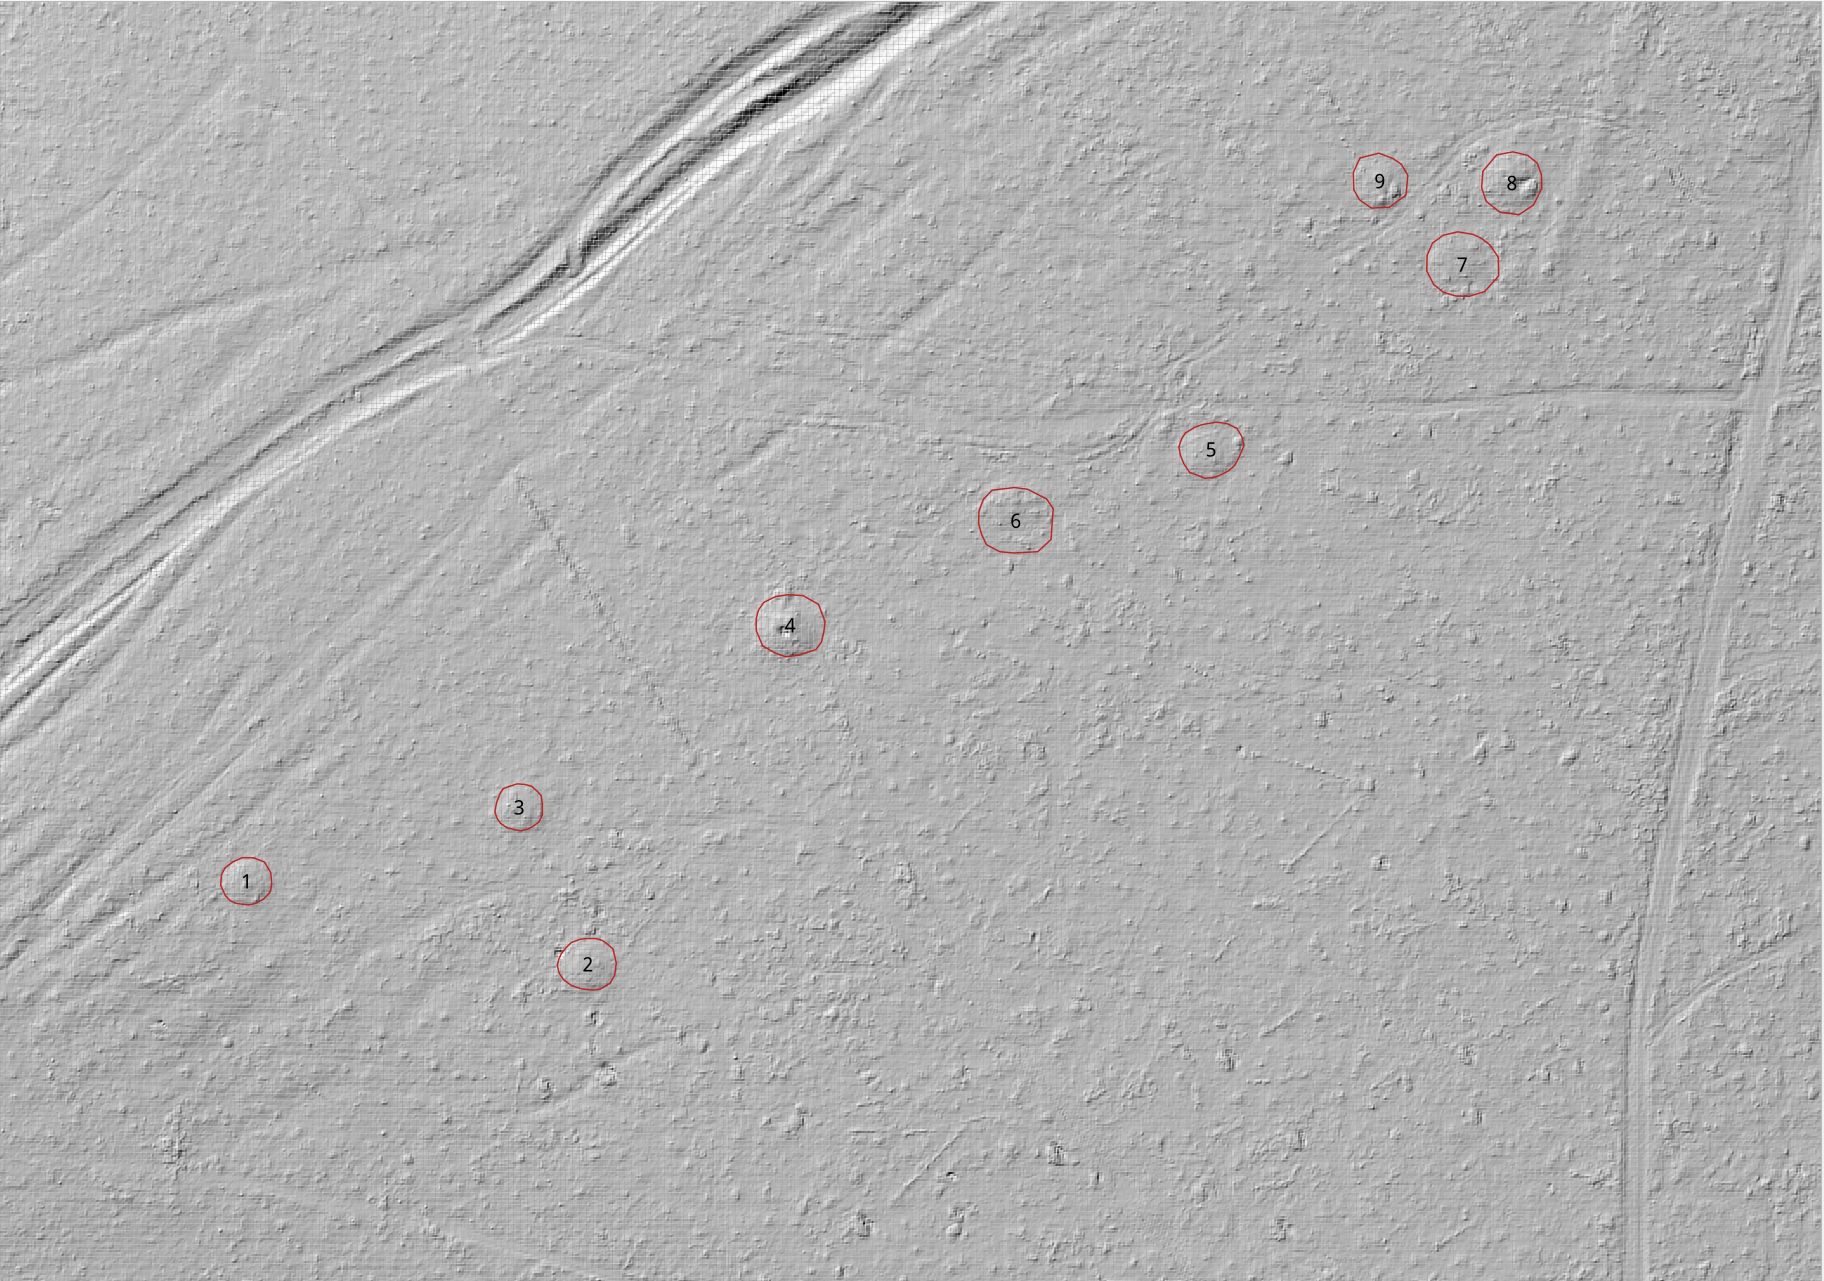
\includegraphics[width=0.5\linewidth,height=0.5\textheight]{C:/Users/kelto/Documents/iSEGMound/analysis/figures/Figure_71}

\}

\caption{Plotting iSEG WS ta and iSEG mtpi WS ta on the DTM, Scale 1:18000.}

(\#fig:Figure\_71)
\textbackslash end\{figure\}

When ``zooming'' in to the two areas (Figure 73) containing burial mounds, we can see the following:
The Northern are (first image of Figure 74) demonstrates again the advantage of using MSTPI: the Site ID 35 is detected by the iSEG mtpi WS workflow, and also a second possible mound, which was only in the profile very slightly visible. Site ID 9 was also detected (in green), although unknowingly: only after the Whitebox MSTPI was checked against Dobiat et al.~1994, became clear that that segment might be Site ID 9. This workflow is better in detecting mounds in this area than the iSEG WS workflow, which missed Site Id 7-5,7-6,7-7 and 7-9).
Looking at the Southern area (second image of Figure 74), iSEG WS workflow detected from Site ID 14 3 mounds more (14-1, 14-8 and 14-11) than the iSEG mtpi WS workflow, which detected 14-3 (but not detected by iSEG WS).
Although a little less accurate in the southern area, the iSEG mtpi WS workflow is more successful.

\textbackslash begin\{figure\}
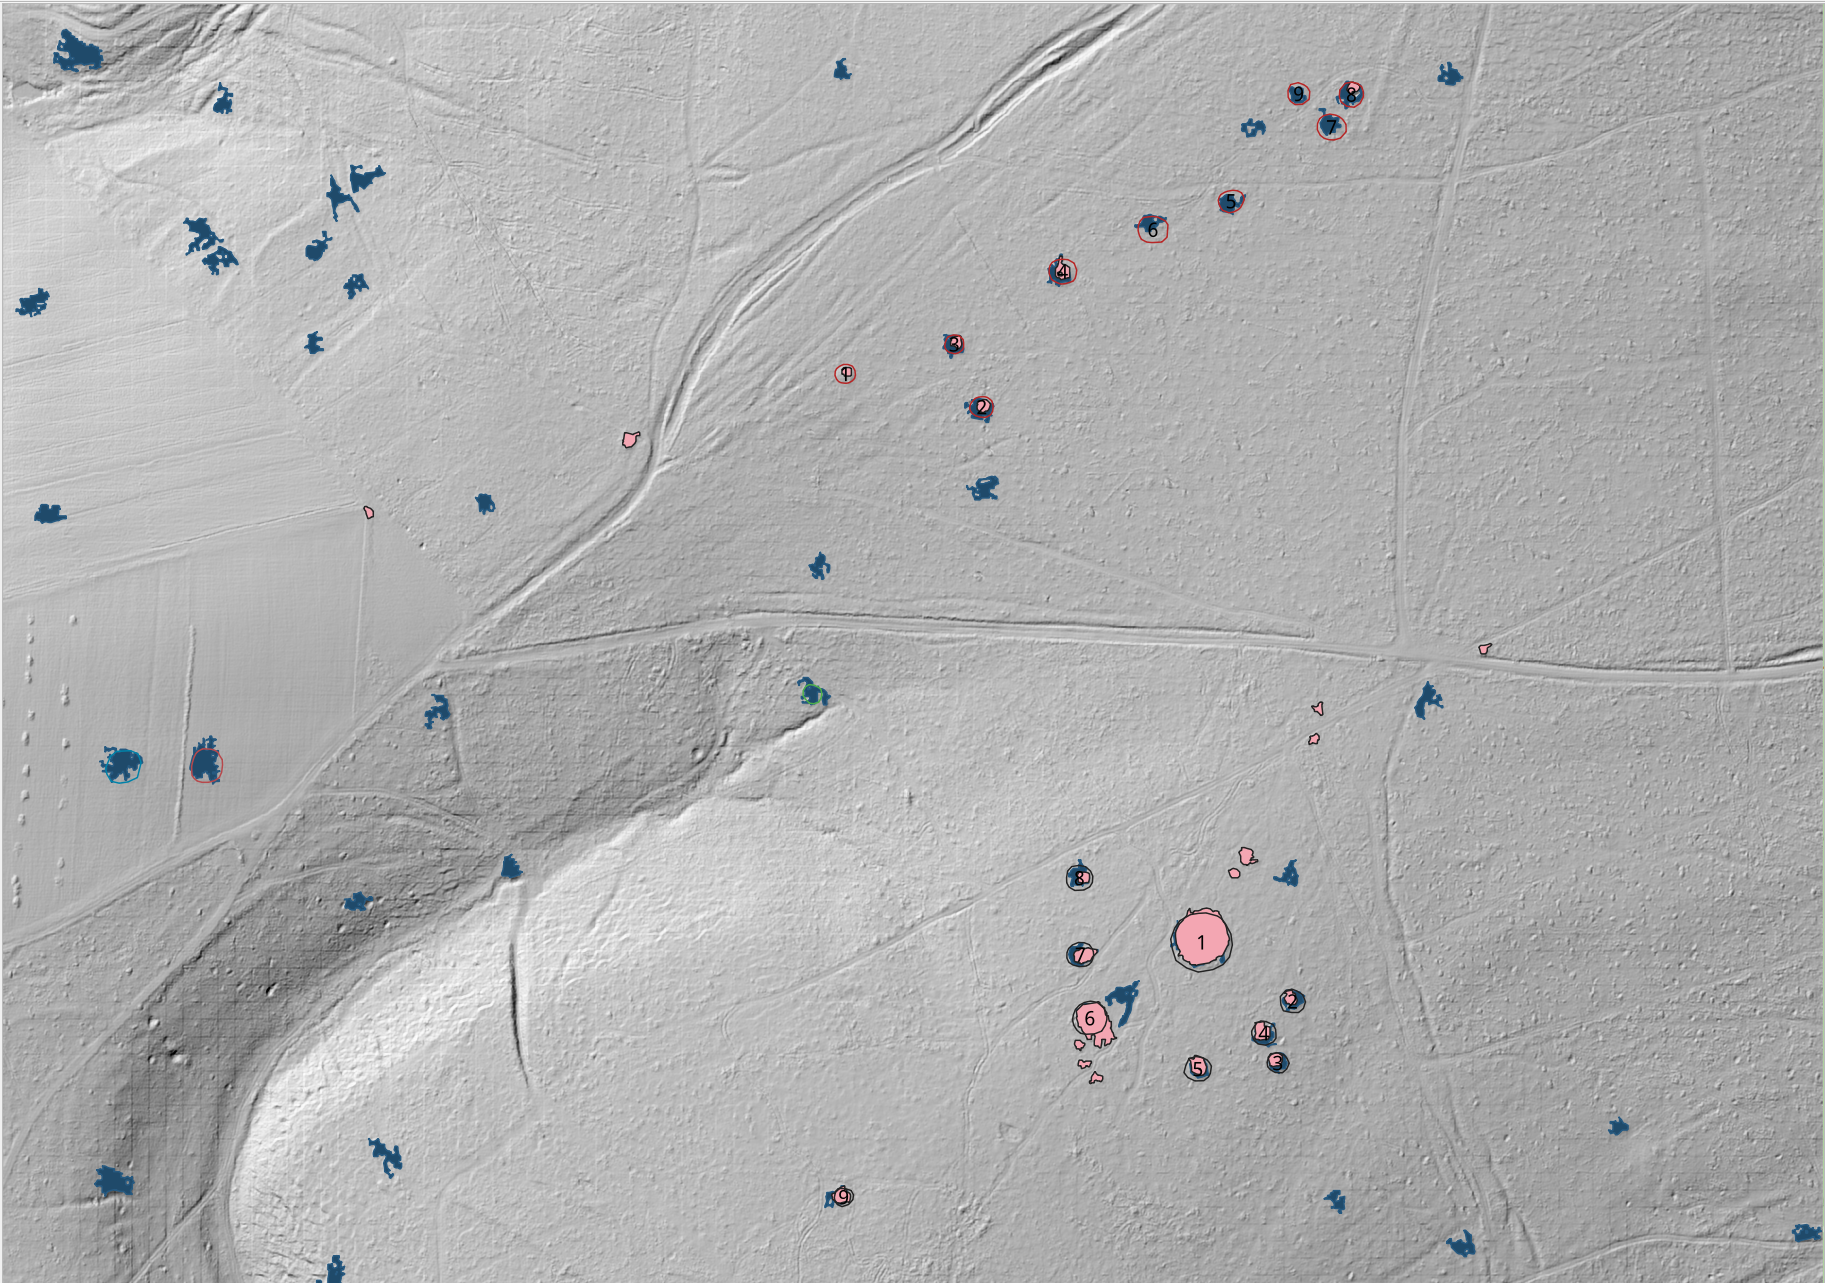
\includegraphics[width=0.5\linewidth]{C:/Users/kelto/Documents/iSEGMound/analysis/figures/Figure_72_1} 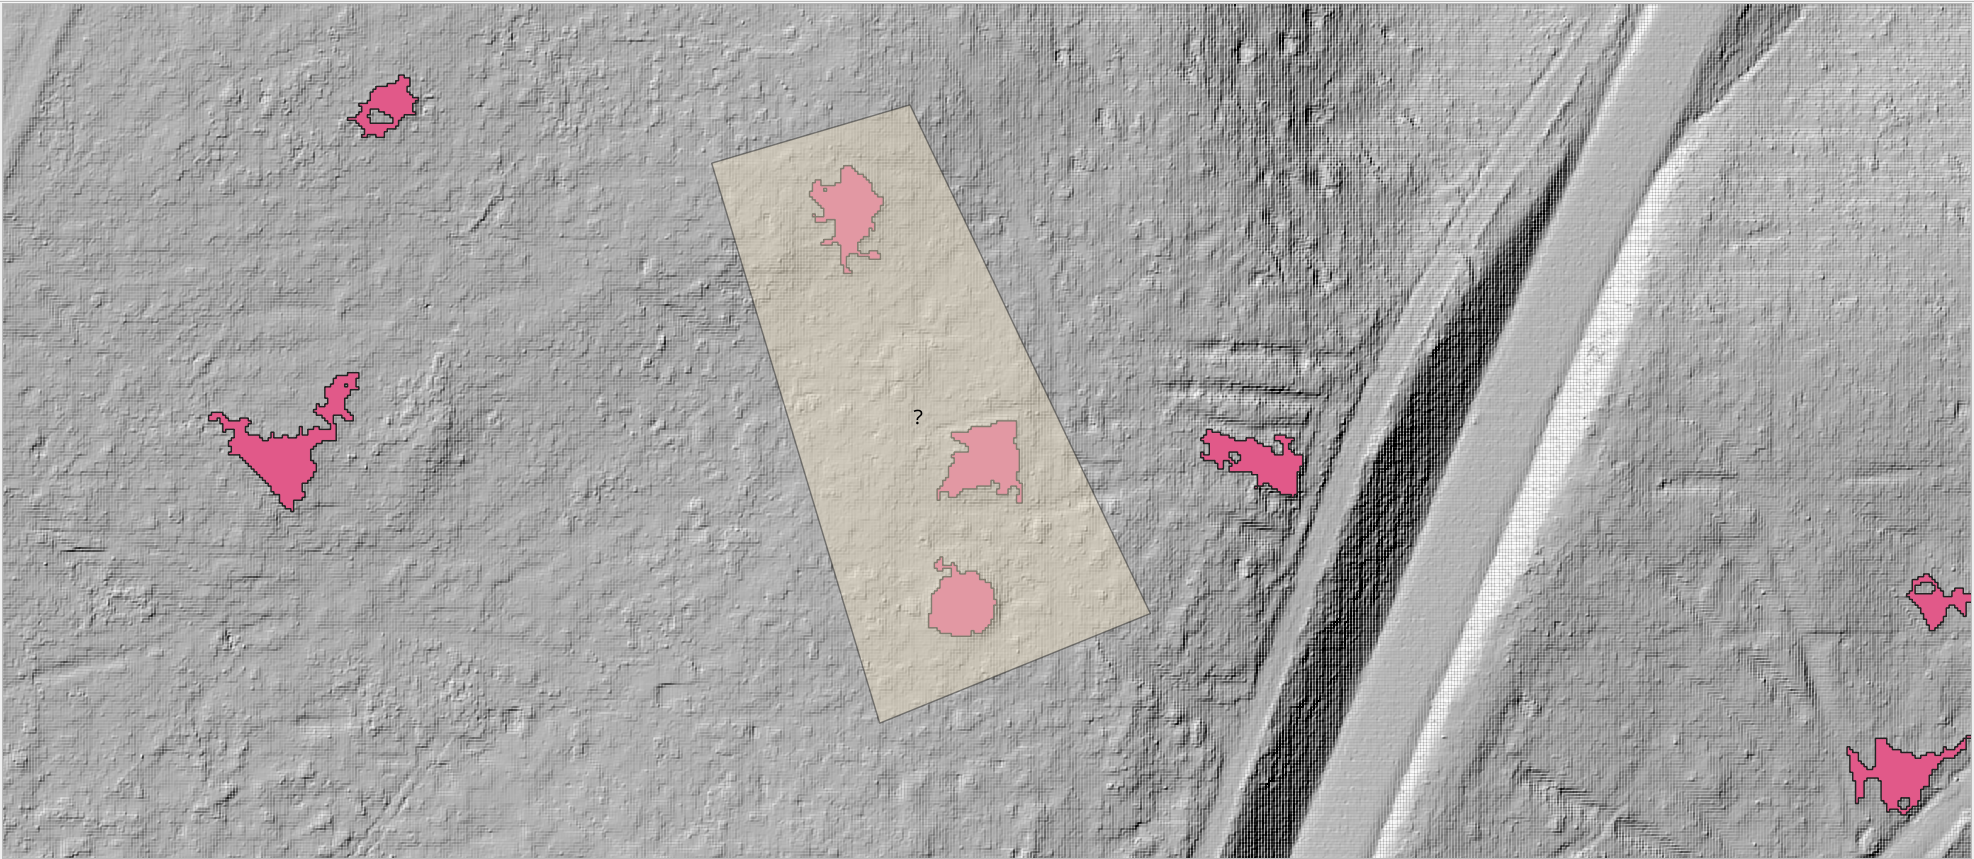
\includegraphics[width=0.5\linewidth]{C:/Users/kelto/Documents/iSEGMound/analysis/figures/Figure_72_2}

\caption{Plotting iSEG WS ta and iSEG mtpi WS ta on the DTM, Scale 1:3000.}

(\#fig:Figure\_72)
\textbackslash end\{figure\}

Considering the Region Growing Segmentation, the overview tells us, that after filtering generally less segments are left over, which fit to \emph{min} to \emph{max} descriptor range as the segments complying to the burial mound mask:

\textbackslash begin\{figure\}

\{\centering 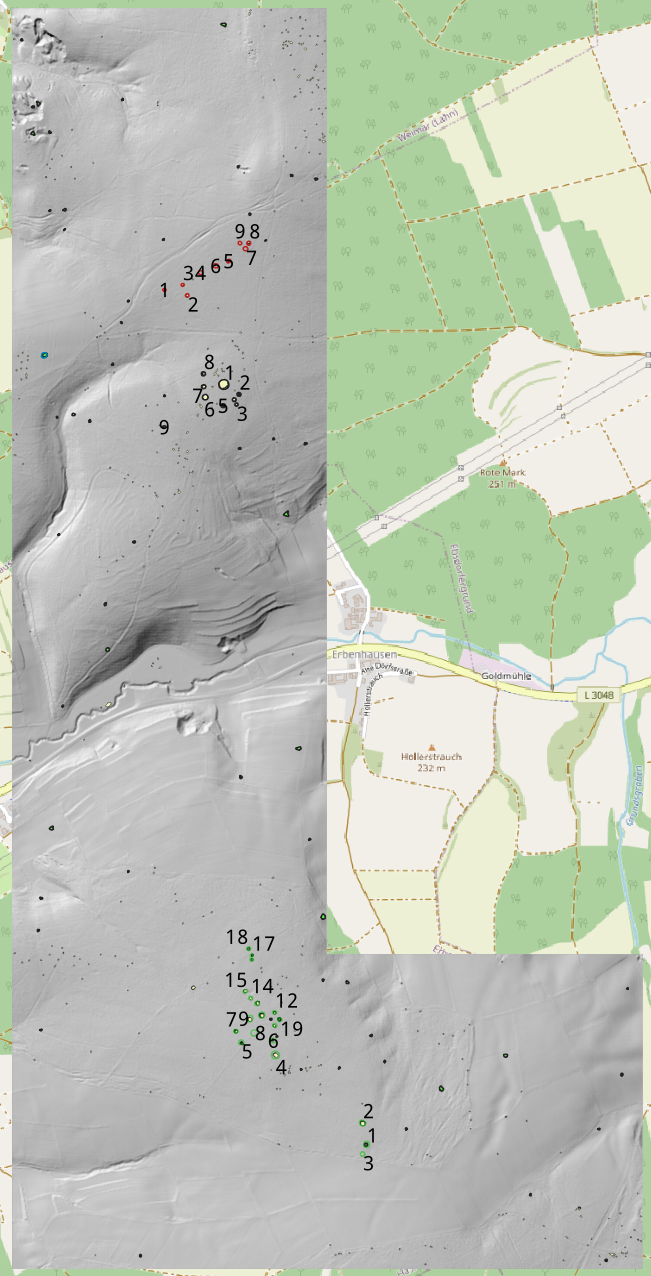
\includegraphics[width=0.5\linewidth,height=0.5\textheight]{C:/Users/kelto/Documents/iSEGMound/analysis/figures/Figure_73}

\}

\caption{Plotting iSEG RG ta and iSEG mtpi RG ta on the DTM, Scale 1:18000.}

(\#fig:Figure\_73)
\textbackslash end\{figure\}

Going into the details, iSEG\_RG\_ta is depicted in lime color and iSEG\_mtpi\_RG in grass green. It is again clear, that using the SAGA MTPI , Site ID 35 is detected, even if only the most visible one.
The iSEG RG workflow does not detect all mounds from Site ID 5 (5-2 is missing and 5-5 is minimally detected), although so far all workflows detected all mounds. In the case of Site ID 7, only 7-1 (at least a part of it), 7-2, 7-3 and 7-8 was detected.
The iSEG mtpi RG workflow did detect all mounds from Site ID 5, but it failed to detect Site ID 7-4, 7-7 and 7-9.
Between the two workflows iSEG mtpi RG is the more successful.

\textbackslash begin\{figure\}
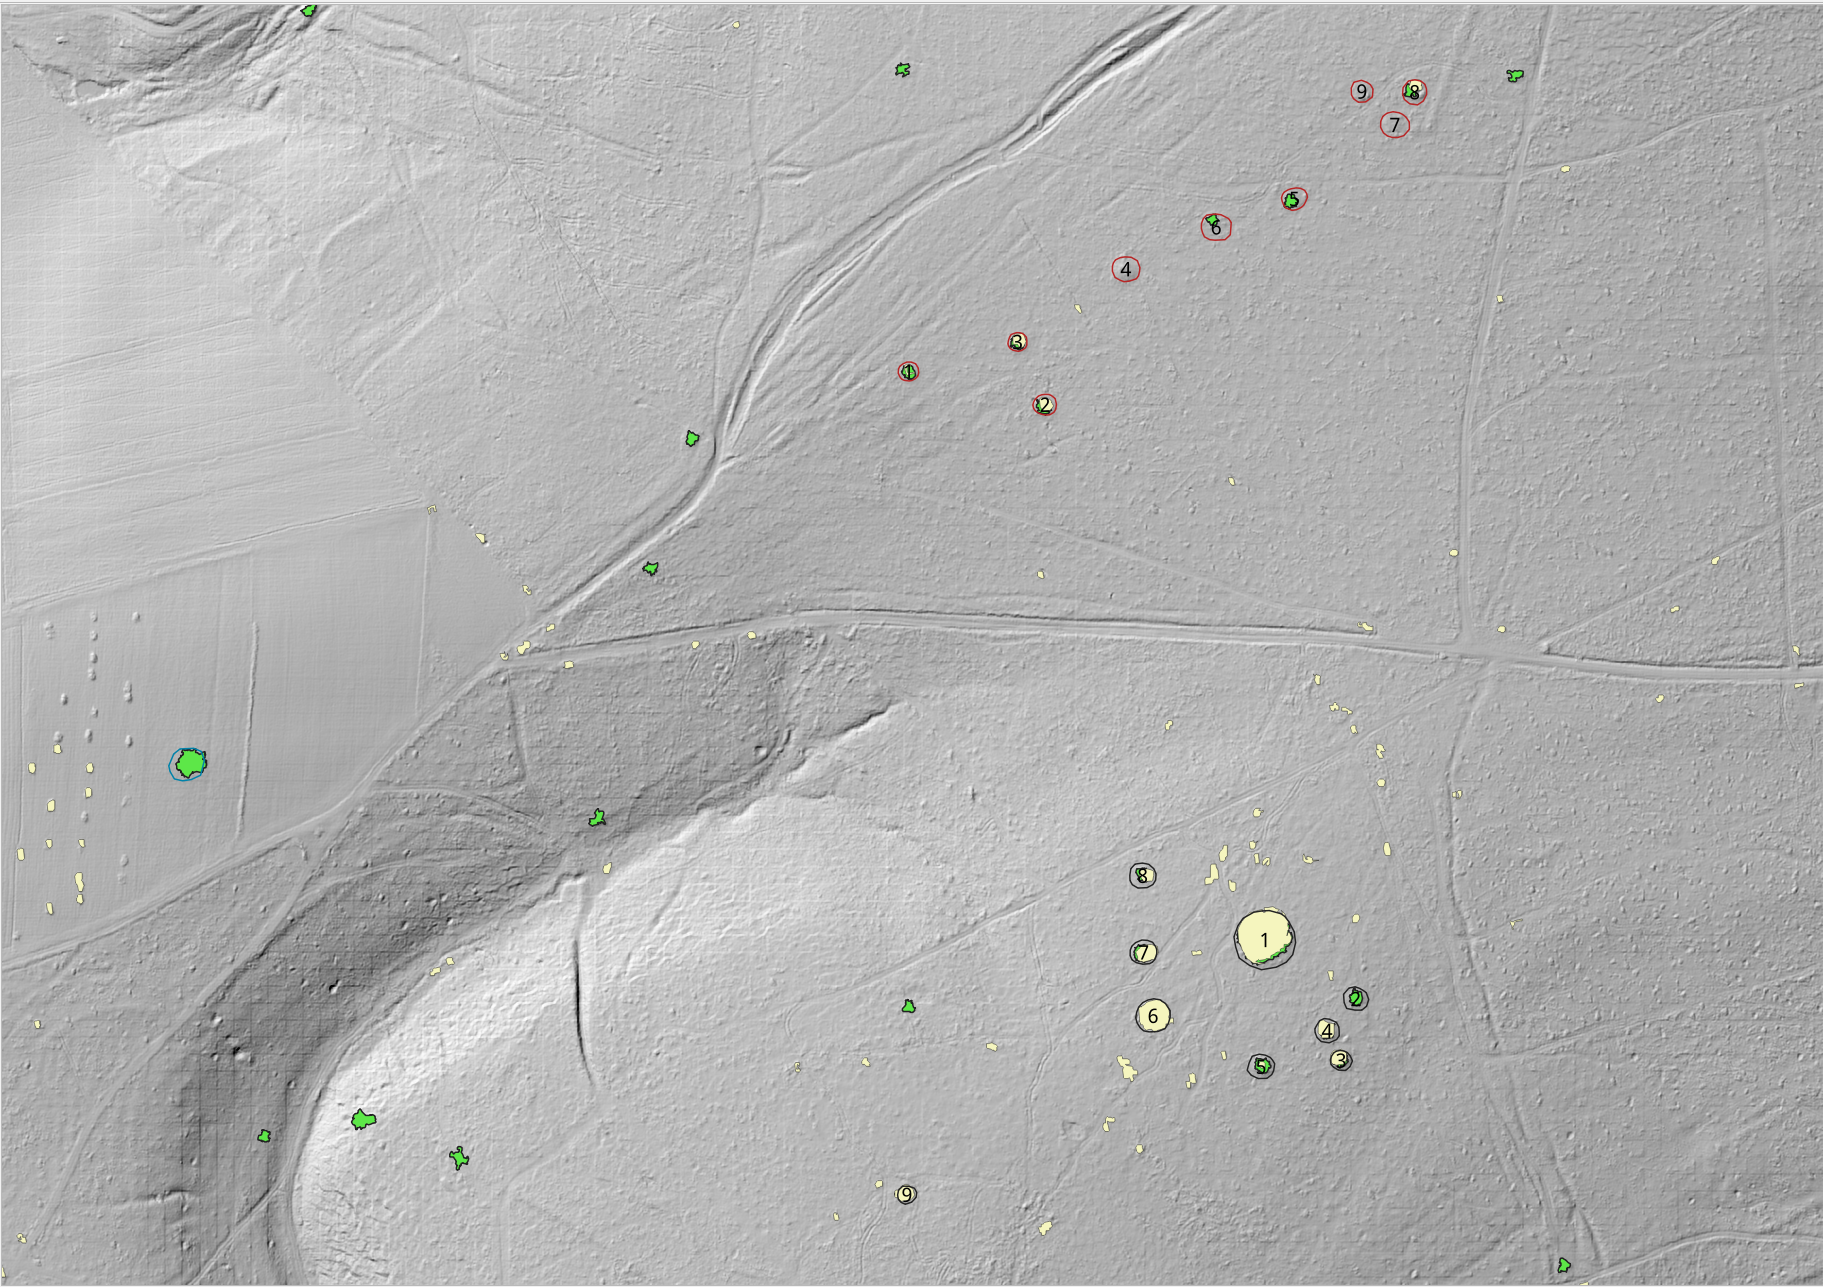
\includegraphics[width=0.5\linewidth]{C:/Users/kelto/Documents/iSEGMound/analysis/figures/Figure_74_1} 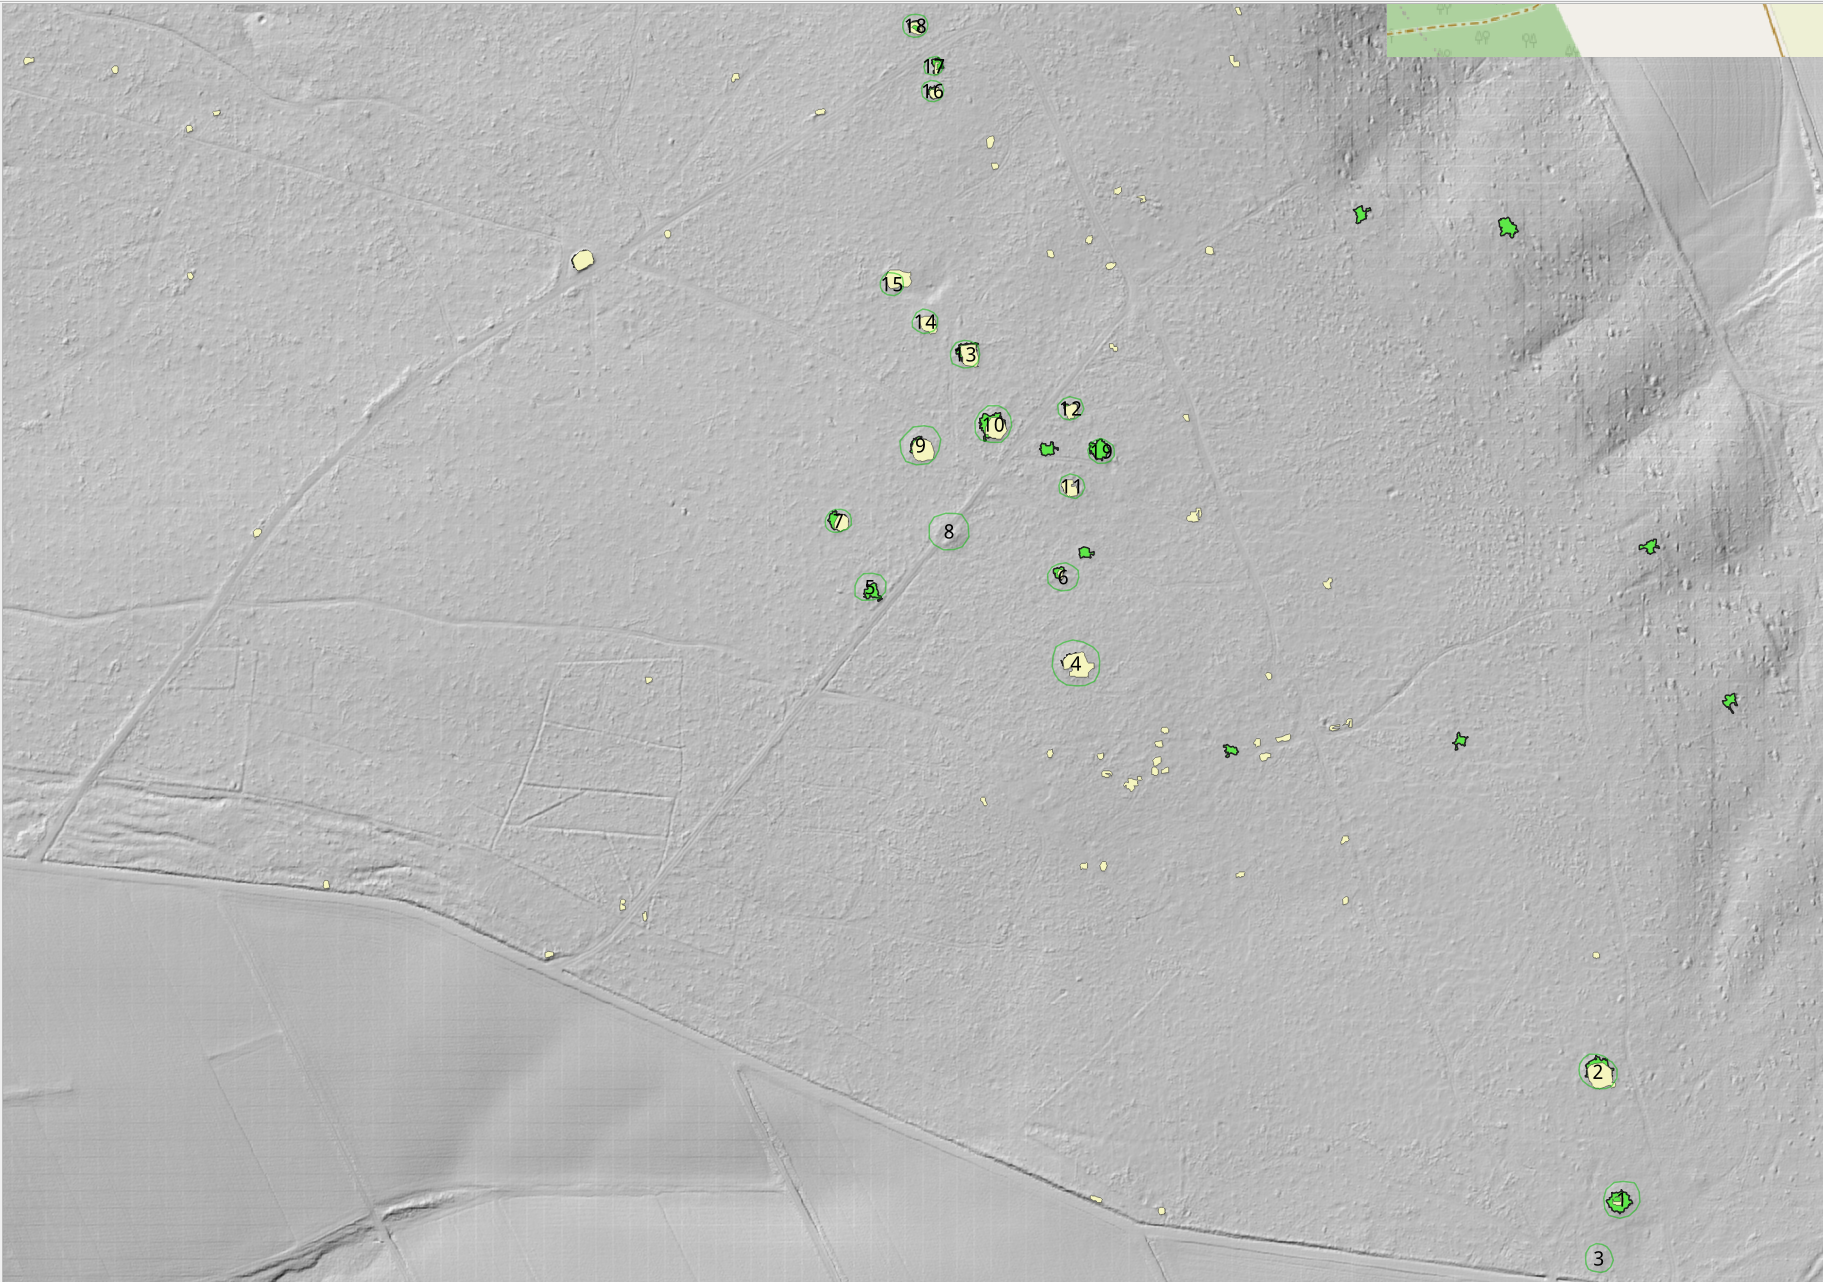
\includegraphics[width=0.5\linewidth]{C:/Users/kelto/Documents/iSEGMound/analysis/figures/Figure_74_2}

\caption{Plotting iSEG RG ta and iSEG mtpi RG ta on the DTM, Scale 1:3000.}

(\#fig:Figure\_74)
\textbackslash end\{figure\}

\newpage

\hypertarget{choosing-the-best-fitting-segmentation}{%
\subsection{\texorpdfstring{\textbf{Choosing the best fitting segmentation}}{Choosing the best fitting segmentation}}\label{choosing-the-best-fitting-segmentation}}

We have seen, that it is clear, that SAGA MTPI as morphometric data preparation methods clearly enhances even the less well visible burial mounds and delineates the mounds more naturally. The remaining question is: how to choose between Watershed and Region growing Segmentation? Which segmentation is better? Two different considerations were investigated: the archaeological decision and the statistical decision.

From the archaeological point of view the aim is to detect as many burial mounds as possible. This can be of course broken down to the question if we want to find the exact shape of the mounds (in the case of the Training DTM and Training Area) or is the most important to detect as much as possible locations in any shape (e.g.~just half or ¾ of a mound is detected) but to detect as many as possible of them. In the case of this Master's, the archaeological choice is definately iSEG\_mtpi\_WS.

The only statistical measure which was found the most approximatively fitting is the \emph{Jaccard Index} or \emph{Intersection over Union}. This measure is used in Deep Learning as an evaluation metric to measure the accuracy of an object detection on the original data set. That is,

\textbackslash begin\{figure\}

\{\centering 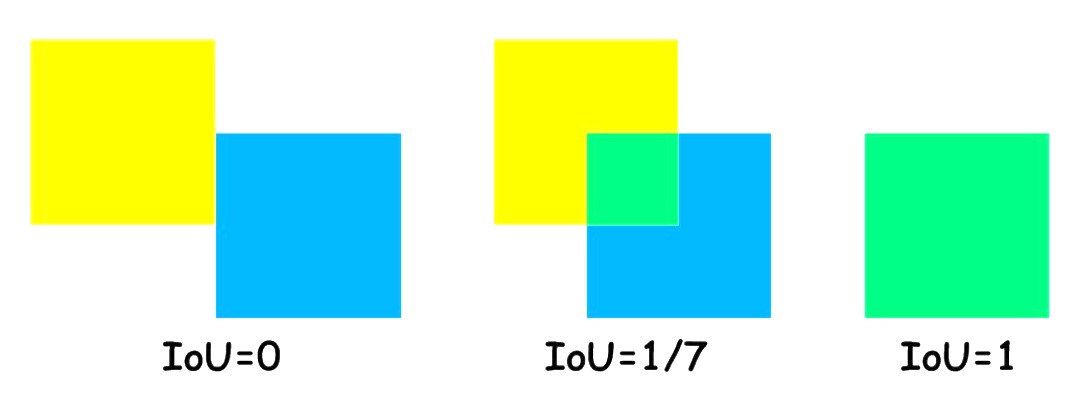
\includegraphics[width=0.5\linewidth,height=0.5\textheight]{C:/Users/kelto/Documents/iSEGMound/analysis/figures/Figure_75}

\}

\caption{Values of Intersection over Union (IoU) or 'Jaccard Index'. Source: https://towardsdatascience.com/intersection-over-union-iou-calculation-for-evaluating-an-image-segmentation-model-8b22e2e84686.}

(\#fig:Figure\_75)
\textbackslash end\{figure\}

\begin{longtable}[t]{llrlr}
\caption{(\#tab:Table 10)Demo table}\\
\toprule
Site\_ID & IoU\_mtpi\_WS & IoU\_mtpi\_RG & SUCCESS & difference\\
\midrule
Site ID 5-1 & 0.7133065 & 0.6916574 & mtpi\_WS & 0.0216491\\
Site ID 5-2 & 0.6003428 & 0.3089561 & mtpi\_WS & 0.2913867\\
Site ID 5-3 & 0.7130259 & 0.4737256 & mtpi\_WS & 0.2393003\\
Site ID 5-4 & 0.5765421 & 0.3383026 & mtpi\_WS & 0.2382395\\
Site ID 5-5 & 0.5115062 & 0.3307759 & mtpi\_WS & 0.1807303\\
\addlinespace
Site ID 5-6 & 0.5890535 & 0.4425936 & mtpi\_WS & 0.1464599\\
Site ID 5-7 & 0.6735597 & 0.4919391 & mtpi\_WS & 0.1816206\\
Site ID 5-8 & 0.5290715 & 0.2553324 & mtpi\_WS & 0.2737391\\
Site ID 5-9 & 0.4605544 & 0.4591942 & mtpi\_WS & 0.0013602\\
Site ID 7-1 & NA & 0.4427740 & mtpi\_RG & NA\\
\addlinespace
Site ID 7-2 & 0.804681 & 0.4973026 & mtpi\_WS & 0.3073784\\
Site ID 7-3 & 0.6831214 & 0.4453112 & mtpi\_WS & 0.2378102\\
Site ID 7-4 & 0.5397044 & NA & mtpi\_WS & NA\\
Site ID 7-5 & 0.5403348 & 0.3031546 & mtpi\_WS & 0.2371802\\
Site ID 7-6 & 0.2942167 & 0.1334789 & mtpi\_WS & 0.1607378\\
\addlinespace
Site ID 7-7 & 0.432601 & NA & mtpi\_WS & NA\\
Site ID 7-8 & 0.6669532 & 0.3527253 & mtpi\_WS & 0.3142279\\
Site ID 7-9 & 0.4702287 & NA & mtpi\_WS & NA\\
Site ID 9 & 0.4634704 & NA & mtpi\_WS & NA\\
Site ID 14-1 & NA & 0.3391305 & mtpi\_RG & NA\\
\addlinespace
Site ID 14-2 & 0.6061152 & 0.5231582 & mtpi\_WS & 0.0829570\\
Site ID 14-3 & 0.5767704 & NA & mtpi\_WS & NA\\
Site ID 14-4 & 0.3778608 & 0.1315178 & mtpi\_WS & 0.2463430\\
Site ID 14-5 & 0.4620573 & 0.2316558 & mtpi\_WS & 0.2304015\\
Site ID 14-6 & NA & 0.1310698 & mtpi\_RG & NA\\
\addlinespace
Site ID 14-7 & 0.6880029 & 0.5178548 & mtpi\_WS & 0.1701481\\
Site ID 14-8 & NA & NA & NA & NA\\
Site ID 14-9 & 0.5652943 & 0.2414775 & mtpi\_WS & 0.3238168\\
Site ID 14-10 & 0.5316726 & 0.4640401 & mtpi\_WS & 0.0676325\\
Site ID 14-11 & NA & 0.2050009 & mtpi\_RG & NA\\
\addlinespace
Site ID 14-12 & 0.5927712 & 0.2642519 & mtpi\_WS & 0.3285193\\
Site ID 14-13 & 0.5579679 & 0.4759892 & mtpi\_WS & 0.0819787\\
Site ID 14-14 & 0.387372 & NA & mtpi\_WS & NA\\
Site ID 14-15 & 0.3837281 & 0.3126799 & mtpi\_WS & 0.0710482\\
Site ID 14-16 & 0.4654447 & 0.2659693 & mtpi\_WS & 0.1994754\\
\addlinespace
Site ID 14-17 & 0.4304659 & 0.3467625 & mtpi\_WS & 0.0837034\\
Site ID 14-18 & NA & 0.2179641 & mtpi\_RG & NA\\
Site ID 14-19 & 0.7427452 & 0.5368112 & mtpi\_WS & 0.2059340\\
Site ID 35-1 & 0.5945741 & 0.5596460 & mtpi\_WS & 0.0349281\\
Site ID 35-2 & 0.6019239 & NA & mtpi\_WS & NA\\
\bottomrule
\end{longtable}

\newpage

\hypertarget{discussion}{%
\section{Discussion}\label{discussion}}

After the technical review of studies which use automation to detect burial mounds and mound-like structures in Archaeological Remote Sensing data sets, the aim of this Master thesis was to detect burial mounds by using the most frequent and easily reproducible methods in the repertoire. As already emphasized in Chapter II and IV, the most accessible workflow is iMound and the only one reproducible workflow in R is published and developed in R (Niculitca 2020). After detailing the framework of the thesis in Chapter III, chapter IV was dedicated to the iSEGMound workflow, the actual product of this Master's thesis.

Although the results of the segmentation(s) are not perfect (often the exact form of the burial mounds is not reached) they still offer a quite effective tool to filter the amount of data to be examined. The input for the workflow can be either a DTM or a MSTPI and from the results of the different workflows it is very clear, that the enhancement of the mounds leads to a better detection (see the case of burial mound group 35, where in the training DTM one and in the training area both mounds are visible), although the mounds can be definitely enhanced better.

Whitebox vs.~SAGA
Technical problems: not updated packages etc.

Shape index is a tricky thing, because the same value can mean different forms

This means on the other hand of course more segments to check, but also more possibility to find previously not known mounds. This will be investigated in the Discussion.

\newpage

\hypertarget{conclusion}{%
\section{Conclusion}\label{conclusion}}

Was haben wir aus der Arbeit gelernt? Hat es funktioniert? Was nicht? Wieso? War es erfolgreich?

Without reproducibility it is hard to really understand and recreate workflows, thus a reproducible workflow like the one developed in this Master's thesis can facilitate the understanding and utilization of automated analysis also by less technically trained archaeologists. It can also enable the joint further development by other specialists and also the reuse of parts of the workflow and knowledge.

The archaeological significance of such a reproducible workflow is moreover the assistance in the analysis of archaeological big datasets not only for research purposes but also for the Cultural Heritage Management sector. Of course the human operator cannot be removed from the equation and has an integral part in providing the variable settings for the different functions in the workflow (as in the case of this Master's thesis), which can be generalized but the different amount of input data (number of tiles) calls for different variable settings which frequently have to be checked.
Using iMound as the first step when looking for burial mounds but basically any archaeological objects which protrude above the ground reduces the amount of data needed to feed to the GeOBIA algorithm. Thus iMound could be used as a useful data extraction method as data preparation in projects with big areas to cover.

\newpage

\hypertarget{bibliography}{%
\section{Bibliography}\label{bibliography}}

\newpage

\hypertarget{supplements}{%
\section{Supplements}\label{supplements}}

\begin{longtable}[t]{rlll}
\caption{(\#tab:Table_2)Table 2: }\\
\toprule
Site\_ID & Dobiat.\_et\_al\_1994 & DTM05 & AoI\\
\midrule
1 & 13 mounds, some are still visible & 12? visible & 4\\
2 & 12 mounds & 11-12? visible & 4\\
3 & 5 + 2 mounds, not visible any more & 5 + 1 + 1 visible & 4\\
4 & 5 mounds & 2 mounds visible? & 4\\
5 & 8 mounds, some are still visible & 9 visible & 4/training area\\
\addlinespace
6 & 5 mounds & 3? visible & 4\\
7 & 15 mounds, some are still visible & 9 visible & 4/training area\\
8 & 7 mounds & 4 visible & 4\\
9 & 2 mounds & 1 visible in WB\_MTPI & 4/training area\\
10 & 8 mounds & 4 visible? & 4\\
\addlinespace
11 & 2 mounds & 2 visible & 4\\
12 & orig. 20 mounds, only few visible & \textasciitilde{} 12 visible & 4\\
13 & 1 mound & 2 visible? & 4\\
14 & 19 mounds & 19 visible & 4/training area\\
15 & 2 + 8 mounds & 2? visible & 4\\
\addlinespace
16 & 4 flat mounds, hardly visible & ? & 3\\
17 & 13 mounds & 10? visible & 3\\
18 & 3 mounds & destroyed & 4\\
19 & 5 mounds & destroyed? & 3\\
20 & ? mounds & ? & 3\\
\addlinespace
21 & 7 mounds & 3 visible & 3\\
22 & \textasciitilde{} 30 mounds? not clear if mounds & \textasciitilde{} 20 visible & 3\\
23 & 17 mounds & \textasciitilde{} 11 visible & 3\\
24 & 1 mound & 2? mounds & 3\\
25 & ? mounds & ? & 3\\
\addlinespace
26 & 6 mounds & ? & 3\\
27 & 3 mounds, destroyed? & destroyed by road? & 3\\
28 & 34 mounds, not all existent & \textasciitilde{} 17? & 3\\
29 & at least 3 mounds & 5? & 3\\
30 & 1 mound & destroyed by road? & 2\\
\addlinespace
31 & ? mounds & ? & 2\\
32 & 1 mound? & 1 visible & 2\\
33 & 1 mound & ? & 2\\
34 & 1 mound & 1+1 bit N ? & 2\\
35 & 2 mounds in the field, ploughed & in WB\_MTPI visible & 4/training area\\
\addlinespace
49 & 2x2 mounds & 2x2 mounds & 1\\
51 & 1 + 2 mounds & 1 + 2 mounds & 1\\
61 & 2 mounds & 2 mounds & 1\\
\bottomrule
\end{longtable}

\begin{longtable}[t]{llllll}
\caption{(\#tab:Table_3)Table 3: Code snipets for processing derivatives in R}\\
\toprule
Derivative & RGRASS.. & whitebox.. & raster.. & spatialEco.. & RSAGA..\\
\midrule
59 Local Relief Model & r.local.relief &  &  &  & \\
52-57 Max Elevation Deviation: local, meso, broad scale &  & wbt\_max\_elevation\_deviation &  &  & \\
35-36 Deviation from Trend &  &  &  & raster.deviation (type = “trend”, global = TRUE/FALSE) & \\
37-38 Deviation from Minimum &  &  &  & raster.deviation (type = “min”, global = TRUE/FALSE) & \\
39-40 Deviation from Maximum &  &  &  & raster.deviation (type = “max”, global = TRUE/FALSE) & \\
\addlinespace
41-42 Deviation from Mean &  &  &  & raster.deviation (type = “mean”, global = TRUE/FALSE) & \\
43 Deviation from Median &  &  &  & raster.deviation (type = “median”, global = FALSE) & \\
44-45 Deviation from SD &  &  &  & raster.deviation (type = “sd”, global = TRUE/FALSE) & \\
58 Multiscale Topographic Index &  & wbt\_multiscale\_topographic\_position\_image &  &  & \\
85-89 Multi-Scale Topographic Index &  &  &  &  & ta\_morphometry module 28\\
\addlinespace
1-2 sum filter &  &  & focal(fun = sum) &  & \\
3-4 min filter &  &  & focal(fun = min) &  & \\
5-6 max filter &  &  & focal(fun = max) &  & \\
7-8 mean filter &  &  & focal(fun = mean) &  & \\
9-10 median filter &  &  & focal(fun = median) &  & \\
\addlinespace
11-12 modal filter &  &  & focal(fun = modal) &  & \\
13-14 sd filter &  &  & focal(fun = sd) &  & \\
15-16 sobel (horizontal \& vertical) f &  &  & focal(fun = sobel) &  & \\
47 Sobal intensity filter &  &  &  & sobal(method = “intensity”) & \\
48 Sobal direction filter &  &  &  & sobal(method = “direction”) & \\
\addlinespace
49 Sobal edge filter &  &  &  & sobal(method = “edge”) & \\
46 Gaussian Smoothing filter &  &  &  & raster.gaussian.smooth() & \\
17/23/66 Terrain Ruggedness Index &  &  & terrain(opt = “TRI”) & tri() & ta\_morphometry module 16\\
18/24 Topographic Position Index &  &  & terrain(opt = “TPI”) & tpi() & \\
19 Roughness &  &  & terrain(opt = “roughness”) &  & \\
\addlinespace
20/71 Slope &  &  & terrain(opt = “slope”) &  & ta\_morphometry module 23\\
21/72 Aspect &  &  & terrain(opt = “aspect”) &  & ta\_morphometry module 23\\
22 Flowdirection &  &  & terrain(opt = “flowdir”) &  & \\
25/67 Vector Ruggedness Measure &  &  &  & vrm() & ta\_morphometry module 17\\
26/73 Profile Curvature &  &  &  & curvature(type = “profile”) & ta\_morphometry module 23\\
\addlinespace
27 Total Curvature &  &  &  & curvature(type = “total”) & \\
28 McNab Curvature &  &  &  & curvature(type = “mcnab”) & \\
29 Boldstad Curvature &  &  &  & curvature(type = “bolstad”) & \\
30 Surface Relief Ratio &  &  &  & srr() & \\
31 Surface Area Ratio &  &  &  & sar() & \\
\addlinespace
32 Dissection &  &  &  & dissection & \\
33 Hierarchical Slope Position &  &  &  & hsp() & \\
34 Raster Multidimensional Scaling &  &  &  & raster.mds & \\
50 Spherical Variance of Surface &  &  &  & spherical.sd(variance = FALSE) & \\
51 Standard Deviation of Surface &  &  &  & spherical.sd(variance = TRUE) & \\
\addlinespace
 &  &  &  &  & lib = “ta\_morphometry”\\
60 Convergence Index &  &  &  &  & module 2 Convergence Index (Search Radius)\\
61 Slope Height &  &  &  &  & module 14 Relative Heights \& Slope Positions\\
62 Valley Depth &  &  &  &  & module 14 Relative Heights \& Slope Positions\\
63 Normalized Height &  &  &  &  & module 14 Relative Heights \& Slope Positions\\
\addlinespace
64 Standardized Height &  &  &  &  & module 14 Relative Heights \& Slope Positions\\
65 Mid-Slope Position &  &  &  &  & module 14 Relative Heights \& Slope Positions\\
68 Terrain Surface Texture       
       resampled &  &  &  &  & module 20 Terrain Surface Texture\\
69 Terrain Surface Texture 
      counting cells &  &  &  &  & module 20 Terrain Surface Texture\\
70 Terrain Surface Convexity &  &  &  &  & module 21 Terrain Surface Convexity\\
\addlinespace
74 Plan Curvature &  &  &  &  & module 23 Morphometric Features\\
75 Longitudinal Curvature &  &  &  &  & module 23 Morphometric Features\\
76 Cross-Sectional Curvature &  &  &  &  & module 23 Morphometric Features\\
77 Maximum Curvature &  &  &  &  & module 23 Morphometric Features\\
78 Minimum Curvature &  &  &  &  & module 23 Morphometric Features\\
\addlinespace
79 Local Curvature &  &  &  &  & module 26 Upslope/Downslope Curvature\\
80 Upward Curvature &  &  &  &  & module 26 Upslope/Downslope Curvature\\
81 Upward Local Curvature &  &  &  &  & module 26 Upslope/Downslope Curvature\\
82 Down Curvature &  &  &  &  & module 26 Upslope/Downslope Curvature\\
83 Downward Local Curvature &  &  &  &  & module 26 Upslope/Downslope Curvature\\
\addlinespace
84 Wind Exposition Index &  &  &  &  & module 27 Wind Exposition Index\\
 &  &  &  &  & lib = “ta\_hydrology”\\
90 SAGA Wetness index &  &  &  &  & module 15 SAGA Wetness Index\\
 &  &  &  &  & lib = “ta\_lightning”\\
91 Negative Openness &  &  &  &  & module 5 Topographic Openness\\
\bottomrule
\end{longtable}

\newpage

\hypertarget{colophon}{%
\section{Colophon}\label{colophon}}

This report was generated on 2021-09-16 18:56:24 using the following computational environment and dependencies:

\begin{Shaded}
\begin{Highlighting}[]
\CommentTok{\# which R packages and versions?}
\ControlFlowTok{if}\NormalTok{ (}\StringTok{"devtools"} \SpecialCharTok{\%in\%} \FunctionTok{installed.packages}\NormalTok{()) devtools}\SpecialCharTok{::}\FunctionTok{session\_info}\NormalTok{()}
\end{Highlighting}
\end{Shaded}

\begin{verbatim}
## - Session info ---------------------------------------------------------------
##  setting  value                       
##  version  R version 4.1.1 (2021-08-10)
##  os       Windows 10 x64              
##  system   x86_64, mingw32             
##  ui       RTerm                       
##  language (EN)                        
##  collate  German_Germany.1252         
##  ctype    German_Germany.1252         
##  tz       Europe/Berlin               
##  date     2021-09-16                  
## 
## - Packages -------------------------------------------------------------------
##  package     * version date       lib source                           
##  assertthat    0.2.1   2019-03-21 [1] CRAN (R 4.1.0)                   
##  bookdown      0.24.1  2021-09-12 [1] Github (rstudio/bookdown@7ce6dc6)
##  cachem        1.0.6   2021-08-19 [1] CRAN (R 4.1.1)                   
##  callr         3.7.0   2021-04-20 [1] CRAN (R 4.1.0)                   
##  cli           3.0.1   2021-07-17 [1] CRAN (R 4.1.0)                   
##  colorspace    2.0-2   2021-06-24 [1] CRAN (R 4.1.0)                   
##  crayon        1.4.1   2021-02-08 [1] CRAN (R 4.1.0)                   
##  DBI           1.1.1   2021-01-15 [1] CRAN (R 4.1.0)                   
##  desc          1.3.0   2021-03-05 [1] CRAN (R 4.1.0)                   
##  devtools      2.4.2   2021-06-07 [1] CRAN (R 4.1.0)                   
##  digest        0.6.27  2020-10-24 [1] CRAN (R 4.1.0)                   
##  dplyr       * 1.0.7   2021-06-18 [1] CRAN (R 4.1.0)                   
##  ellipsis      0.3.2   2021-04-29 [1] CRAN (R 4.1.0)                   
##  evaluate      0.14    2019-05-28 [1] CRAN (R 4.1.0)                   
##  fansi         0.5.0   2021-05-25 [1] CRAN (R 4.1.0)                   
##  farver        2.1.0   2021-02-28 [1] CRAN (R 4.1.0)                   
##  fastmap       1.1.0   2021-01-25 [1] CRAN (R 4.1.0)                   
##  fs            1.5.0   2020-07-31 [1] CRAN (R 4.1.0)                   
##  generics      0.1.0   2020-10-31 [1] CRAN (R 4.1.0)                   
##  ggplot2     * 3.3.5   2021-06-25 [1] CRAN (R 4.1.0)                   
##  glue          1.4.2   2020-08-27 [1] CRAN (R 4.1.0)                   
##  gtable        0.3.0   2019-03-25 [1] CRAN (R 4.1.0)                   
##  here          1.0.1   2020-12-13 [1] CRAN (R 4.1.0)                   
##  htmltools     0.5.2   2021-08-25 [1] CRAN (R 4.1.1)                   
##  knitr         1.34    2021-09-09 [1] CRAN (R 4.1.1)                   
##  labeling      0.4.2   2020-10-20 [1] CRAN (R 4.1.0)                   
##  lifecycle     1.0.0   2021-02-15 [1] CRAN (R 4.1.0)                   
##  magrittr      2.0.1   2020-11-17 [1] CRAN (R 4.1.0)                   
##  memoise       2.0.0   2021-01-26 [1] CRAN (R 4.1.0)                   
##  morris        0.0.0.1 2021-09-02 [1] Github (cshoggard/morris@4364adf)
##  munsell       0.5.0   2018-06-12 [1] CRAN (R 4.1.0)                   
##  pillar        1.6.2   2021-07-29 [1] CRAN (R 4.1.0)                   
##  pkgbuild      1.2.0   2020-12-15 [1] CRAN (R 4.1.0)                   
##  pkgconfig     2.0.3   2019-09-22 [1] CRAN (R 4.1.0)                   
##  pkgload       1.2.2   2021-09-11 [1] CRAN (R 4.1.1)                   
##  png           0.1-7   2013-12-03 [1] CRAN (R 4.1.0)                   
##  prettyunits   1.1.1   2020-01-24 [1] CRAN (R 4.1.0)                   
##  processx      3.5.2   2021-04-30 [1] CRAN (R 4.1.0)                   
##  ps            1.6.0   2021-02-28 [1] CRAN (R 4.1.0)                   
##  purrr         0.3.4   2020-04-17 [1] CRAN (R 4.1.0)                   
##  R6            2.5.1   2021-08-19 [1] CRAN (R 4.1.1)                   
##  remotes       2.4.0   2021-06-02 [1] CRAN (R 4.1.0)                   
##  rlang         0.4.11  2021-04-30 [1] CRAN (R 4.1.0)                   
##  rmarkdown     2.11    2021-09-14 [1] CRAN (R 4.1.1)                   
##  rprojroot     2.0.2   2020-11-15 [1] CRAN (R 4.1.0)                   
##  rstudioapi    0.13    2020-11-12 [1] CRAN (R 4.1.0)                   
##  scales        1.1.1   2020-05-11 [1] CRAN (R 4.1.0)                   
##  sessioninfo   1.1.1   2018-11-05 [1] CRAN (R 4.1.0)                   
##  stringi       1.7.4   2021-08-25 [1] CRAN (R 4.1.1)                   
##  stringr       1.4.0   2019-02-10 [1] CRAN (R 4.1.0)                   
##  testthat      3.0.4   2021-07-01 [1] CRAN (R 4.1.0)                   
##  tibble        3.1.4   2021-08-25 [1] CRAN (R 4.1.1)                   
##  tidyselect    1.1.1   2021-04-30 [1] CRAN (R 4.1.0)                   
##  usethis       2.0.1   2021-02-10 [1] CRAN (R 4.1.0)                   
##  utf8          1.2.2   2021-07-24 [1] CRAN (R 4.1.0)                   
##  vctrs         0.3.8   2021-04-29 [1] CRAN (R 4.1.0)                   
##  withr         2.4.2   2021-04-18 [1] CRAN (R 4.1.0)                   
##  xfun          0.26    2021-09-14 [1] CRAN (R 4.1.1)                   
##  yaml          2.2.1   2020-02-01 [1] CRAN (R 4.1.0)                   
## 
## [1] C:/Users/kelto/Documents/R/win-library/4.1
## [2] C:/Program Files/R/R-4.1.1/library
\end{verbatim}

The current Git commit details are:

\begin{Shaded}
\begin{Highlighting}[]
\CommentTok{\# what commit is this file at? }
\ControlFlowTok{if}\NormalTok{ (}\StringTok{"git2r"} \SpecialCharTok{\%in\%} \FunctionTok{installed.packages}\NormalTok{() }\SpecialCharTok{\&}\NormalTok{ git2r}\SpecialCharTok{::}\FunctionTok{in\_repository}\NormalTok{(}\AttributeTok{path =} \StringTok{"."}\NormalTok{)) git2r}\SpecialCharTok{::}\FunctionTok{repository}\NormalTok{(here}\SpecialCharTok{::}\FunctionTok{here}\NormalTok{())  }
\end{Highlighting}
\end{Shaded}

\begin{verbatim}
## Local:    main C:/Users/kelto/Documents/iSEGMound
## Remote:   main @ origin (https://github.com/keltoskytoi/iSEGMound)
## Head:     [db31def] 2021-09-15: couldn't leave it alone...
\end{verbatim}

\end{document}
